%---------------------------------------------------------------------
%  Writeup of the latest and  greatest search of Run II data for
%  single top quark production at DZero.
%  Started 08/31/06
%  Continued 10/14/06
%  Authors: The Single Top Working Group
%
%---------------------------------------------------------------------
%
\documentclass[aps]{revtex4}

% Allow figures to be included
\usepackage{graphicx}

% Allow type to be colored (68 colors)
\usepackage[usenames]{color}

% Allow rotation of tables, figures, pages
\usepackage{rotating}

% Add a gray bar to the margin for new text
\usepackage{changebar}

% Allow sub figures
\usepackage{subfigure}

% Fix too narrow margins
\paperheight 11 in
\paperwidth 8.5 in
\textwidth 6.5 in
\oddsidemargin 0 pt
\marginparsep 0 pt
\marginparwidth 0 pt
\voffset 0 in
\hoffset 0 in

% Fix hard-to-follow section numbering
\renewcommand{\thesection}
{\Large\arabic{section}}
\renewcommand{\thesubsection}
{\large\arabic{section}.\large\arabic{subsection}}
\renewcommand{\thesubsubsection}
{\arabic{section}.\arabic{subsection}.\arabic{subsubsection}}
\renewcommand{\theparagraph}
{\arabic{section}.\arabic{subsection}.\arabic{subsubsection}.\arabic{paragraph}}

% Change the table numbering from roman to arabic
\renewcommand{\thetable}{\arabic{table}}

% Fix problems with font changes after a reference to a section 
\let\LaTEXref\ref
\renewcommand{\ref}[1]
{{\LaTEXref{#1}}}

% Make section titles size match text size
\makeatletter
\renewcommand{\section}{\@startsection
	{section}%
	{1}%
	{0pt}%
	{-\baselineskip}%
	{1.0\baselineskip}%
	{\center\bfseries\Large\rmfamily\scshape}}%
\renewcommand{\subsection}{\@startsection
	{subsection}%
	{2}%
	{0pt}%
	{-\baselineskip}%
	{1.0\baselineskip}%
	{\center\bfseries\large\rmfamily}}%
\renewcommand{\subsubsection}{\@startsection
	{subsubsection}%
	{3}%
	{0pt}%
	{-\baselineskip}%
	{1.0\baselineskip}%
	{\center\itshape\large\rmfamily}}%
\renewcommand{\paragraph}{\@startsection
	{paragraph}%
	{4}%
	{0pt}%
	{-\baselineskip}%
	{1.0\baselineskip}%
	{\center\itshape\rmfamily}}%

% Fix references to sections
\renewcommand{\p@subsection}{}
\renewcommand{\p@subsubsection}{}
\renewcommand{\p@paragraph}{}
\renewcommand{\p@subparagraph}{}

\makeatother

% Put page number at bottom of page
\pagestyle{plain}

% Avoid too much hyphenation at the ends of lines
\lefthyphenmin=6
\righthyphenmin=6

% Allow a figure to occupy most of a column without being
% placed on a separate page that includes no text
\renewcommand{\topfraction}      {0.95}
\renewcommand{\bottomfraction}   {0.95}
\renewcommand{\floatpagefraction}{0.95}
\renewcommand{\textfraction}     {0.05}

% Tighten up the itemized lists
\newenvironment{myitemize}{\begin{itemize}
                \setlength{\itemsep}{-1 pt}}{\end{itemize}}

% Tighten up the itemized description lists
\newenvironment{mydescription}{\begin{description}
                \setlength{\itemsep}{-1 pt}}{\end{description}}

% Tighten up the enumerated lists
\newenvironment{myenumerate}{\begin{enumerate}
                \setlength{\itemsep}{-1 pt}}{\end{enumerate}}

% Define some abbreviations
\newcommand{\dzero}     {D\O}
\newcommand{\met}       {\mbox{$\not\!\!E_T$}}
\newcommand{\pt}        {\mbox{$p_{\rm T}$}}
\newcommand{\deta}      {\mbox{$\eta^{\rm det}$}}
\newcommand{\meta}      {\mbox{$\left|\eta\right|$}}
\newcommand{\mdeta}     {\mbox{$\left|\eta^{\rm det}\right|$}}
\newcommand{\rar}       {\rightarrow}
\newcommand{\rargap}    {\mbox{ $\rightarrow$ }}
\newcommand{\tbbar}     {\mbox{$tb$}}
\newcommand{\tqbbar}    {\mbox{$tqb$}}
\newcommand{\ttbar}     {\mbox{$t\bar{t}$}}
\newcommand{\bbbar}     {\mbox{$b\bar{b}$}}
\newcommand{\ccbar}     {\mbox{$c\bar{c}$}}
\newcommand{\qqbar}     {\mbox{$q\bar{q}$}}
\newcommand{\ppbar}     {\mbox{$p\bar{p}$}}
\newcommand{\lepjets}   {\mbox{${\ttbar}{\rar}\ell$+jets}}
\newcommand{\dilepton}  {\mbox{${\ttbar}{\rar}\ell\ell$}}
\newcommand{\comphep}   {\sc{c}\rm{omp}\sc{hep}}
\newcommand{\singletop} {\sc{s}\rm{ingle}\sc{t}\rm{op}}
\newcommand{\herwig}    {\sc{herwig}}
\newcommand{\pythia}    {\sc{pythia}}
\newcommand{\alpgen}    {\sc{alpgen}}
\newcommand{\tauola}    {\sc{tauola}}
\newcommand{\evtgen}    {\sc{e}\rm{vt}\sc{g}\rm{en}}
\newcommand{\reco}      {\sc{reco}}
\newcommand{\pderiv}[2]{\frac{\partial #1}{\partial #2}}
%---------------------------------------------------------------------
%---------------------------------------------------------------------
\begin{document}

\begin{table}
\begin{flushleft}
\begin{minipage}{5.5 in}
\begin{tabular}{lr}
%{\leftline{\includegraphics[scale=0.3]{../figures/d0logo}}}
& \hspace{-0.5in}{\large{\dzero} Note 5287} \\
%{\large For Top Group and EB review}
& \hspace{-0.5in}{\large November 28, 2006} \\
%{\large Comments to d0-run2eb-024@fnal.gov,}
& \hspace{-0.5in}{\large Version 1.2} \\
%{\large Thomas~Gadfort, Aurelio~Juste, Jovan~Mitrevski, John~Parsons,} & \\
%{\large Gordon~Watts, Ar\'{a}n~Garc\'{\i}a-Bellido, and Ann~Heinson} & \\
%{\large {\color{red}{Deadline: Monday, November XX, 2006}}} & \\
\end{tabular}
\end{minipage}
\end{flushleft}
\end{table}



\title{\LARGE{\vspace{0.35in}Search for Single Top Quark Production
Using The Matrix Element Analysis Technique in 1~fb$^{-1}$ of Data}\\
\vspace{0 in}}

%--------
%  Secret title is something like ``New Mode of Top Quark Production
%  Observed at the Tevatron''
%--------

\author{\large{
E.~Aguil\'{o},$^{2}$
P.~Baringer$^{10}$
A.~Bean,$^{10}$
C.~Belanger-Champagne,$^{11}$
J.A.~Benitez,$^{12}$
E.E.~Boos,$^{13}$
R.~Brock,$^{12}$
V.~Bunichev, $^{13}$
K.~Chan,$^{2}$
L.~Christofek,$^{4}$
Y.~Coadou,$^{17}$
L.V.~Dudko,$^{13}$
M.~Erdmann,$^{1}$
T.~Gadfort,$^{18}$
A.~Garc\'{\i}a-Bellido,$^{18}$
C.~Gerber,$^{9}$
D.~Gillberg,$^{17}$
G.~Gutierrez,$^{7}$
P.~Gutierrez,$^{14}$
A.P.~Heinson,$^{5}$
U.~Heintz,$^{3}$
S.~Herrin,$^{16}$
S.~Jabeen,$^{3}$
S.~Jain,$^{14}$
A.~Juste,$^{7}$
S.~Kappler,$^{1}$
D.~Kau,$^{8}$
G.~Kertzscher,$^{11}$
M.~Kirsch,$^{1}$
L.~Li,$^{5}$
J.~Mitrevski,$^{6}$
R.~Moore,$^{2}$
M.~Narain,$^{3,4}$
D.~O'Neil,$^{17}$
M.~Pangilinan,$^{3}$
J.~Parsons,$^{6}$
M.~Perfilov,$^{13}$
C.~Potter,$^{11}$
H.B.~Prosper,$^{8}$
R.~Schwienhorst,$^{12}$
E.~Shabalina,$^{9}$
J.~Steggemann,$^{1}$
T.~Tim,$^{9}$
C.~Tully,$^{15}$
M.~Vetterli,$^{17}$
B.~Vachon,$^{11}$
G.~Watts,$^{18}$
M.~Weber$^{7}$
}}

\affiliation{\large{\vspace*{0.1in}
$^{1}$RWTH Aachen University\\
$^{2}$University of Alberta\\
$^{3}$Boston University\\
$^{4}$Brown University\\
$^{5}$University of California, Riverside\\
$^{6}$Columbia University\\
$^{7}$Fermi National Accelerator Laboratory\\
$^{8}$Florida State University\\
$^{9}$University of Illinois, Chicago\\
$^{10}$University of Kansas\\
$^{11}$McGill University\\
$^{12}$Michigan State University\\
$^{13}$Moscow State University\\
$^{14}$University of Oklahoma\\
$^{15}$Princeton University\\
$^{16}$Rice University\\
$^{17}$Simon Fraser University\\
$^{18}$University of Washington
}}

\begin{abstract}
{\vspace{0.1in}\large{This note describes the application of the
matrix element analysis technique to the search for single top quark
production at {\dzero} using nearly 1~fb$^{-1}$ of Run~II data. From a
comparison of the matrix element discriminants between data and the
background model, we measure the single top quark production
cross section:
$$
\sigma\left({\ppbar}{\rargap}tb+tqb+X\right)
= 4.6 ^{+1.8}_{-1.5}~{\rm pb}
$$ }}

\end{abstract}

\maketitle

%---------------------------------------------------------------------
%---------------------------------------------------------------------
%---------------------------------------------------------------------
%---------------------------------------------------------------------
\clearpage
\tableofcontents
\vfill\eject

\large{

%---------------------------------------------------------------------
\clearpage
%---------------------------------------------------------------------
\section{Introduction}

The search for single top quark production at the Tevatron has turned
out to be a significantly more difficult task than anybody
anticipated. Despite the large production cross section predicted by
the standard model (about half of that for top quark pairs) and the
distinct event signature involving a leptonic $W$ boson decay and two
or more jets (at least one being a $b$~jet), this top quark production
mode has not yet been observed. The main reason is that signal events
are overwhelmed by a background from $W$+jets orders of magnitude
larger. At jet multiplicities above two, even $t\bar{t}$ becomes a
significant background. Both backgrounds can mimic the signal event
characteristics in such a way that no cut on a single distribution can
be used to effectively remove the background while preserving a large
enough signal fraction. However, the combined information from
several discriminant variables in a multivariate approach can
potentially achieve enough sensitivity to unambiguously establish a
signal. By now this is widely acknowledged as a requirement for any
viable search for single top production, and all ongoing analyses at
{\dzero} are of a multivariate nature.

Methods such as neural networks or decision trees are being
succesfully used at D{\O} to build efficient event discriminants to
separate signal from background. These methods rely on identifying an
optimal (and usually very large) set of kinematic and topological
variables that collectively encode most of the available information
to classify signal and background events. These methods are ``learning
machines'' since they adjust to minimize the misclassification rate in
samples of pseudo-data containing pure signal and background events
that are presented to them. In this note we describe the so-called
``Matrix Element-based Single Top Search'' which, as will be explained
below, is intrinsically different in approach.

First of all, the matrix element (ME) method attempts to maximize the
sensitivity to the signal by making exhaustive use of the available
kinematic information in the event, as contained in the four-momenta
for the reconstructed objects. Information regarding $b$~tagging has
also been incorporated in the current version of the analysis. This is
the complete set of variables considered in this analysis. Then,
starting from these four-momenta, this method uses the matrix elements
for the different signal and background processes to numerically
compute the event probability density for each hypothesis (signal and
background). This method has been developed and successfully applied
at {\dzero} in the past for parameter estimation such as the top quark
mass~\cite{Abazov:2004cs,Abazov:2006bd} or the longitudinal $W$~boson
helicity fraction in top quark decays~\cite{Abazov:2004ym}. In this
analysis, the computed event probability densities are used to build
an optimal event discriminant between signal and background,
representing the first application of this method to a search at
{\dzero}.

The analysis described in this note is based on the selected
``lepton+jets'' data samples described in Ref.~\cite{general-note}.
The current analysis is restricted to two-jet and three-jet events,
with at least one of the jets $b$~tagged.

This note is organized as follows. Section~\ref{separation-ME}
presents an overview of the method, from the calculation of the event
probability density functions, to the construction of the different
event discriminants. Section~\ref{data-MC} contains comparisons
between data and the background model for the different event
discriminant distributions from control and signal samples.
Section~\ref{sec:ensembles} presents results of the analysis run on a
number of Monte Carlo ensembles. Section~\ref{exp-performance} is
devoted to a discussion of the expected performance, both in terms of
significance and cross section measurement. Section~\ref{results}
presents the measured results from data, followed by
Section~\ref{sec:eventcharacteristics} which shows characteristics of
the events selected according to their values of the signal
discriminants. Finally, Section~\ref{summary} is devoted to a summary
and conclusions.




\clearpage
%---------------------------------------------------------------------
\section{Separation of Signal from Background Using Matrix Elements}
\label{separation-ME}

\subsection{Method Overview}
\label{method-overview}

The search for single top quark production critically depends on being
able to discriminate between signal-like and background-like events
or, in other words, to perform the optimal test of hypothesis $H_0$:
signal (S), against hypothesis $H_1$: background (B). In this case,
given an event characterized by a set of variables $\vec{x}$, the most
powerful test of hypothesis is given by the Neyman-Pearson test, which
involves a cut on the ratio:
\begin{equation}
\label{disc}
\ell(\vec{x},H_0,H_1) = \frac{P(\vec{x}|H_0)}{P(\vec{x}|H_1)}
= \frac{P_S(\vec{x})}{P_B(\vec{x})},
\end{equation}
\noindent where $P_S(\vec{x})$ and $P_B(\vec{x})$ stand,
respectively, for the signal and background probability density
functions of $\vec{x}$. The power of such a test is also maximal if
the set of variables $\vec{x}$ is complete, in the sense that they
contain all information that is relevant to discriminate between
signal and background. Such optimal test of hypothesis can also be
performed on the a-posteriori Bayesian probability (or Bayes
posterior) of ``$S$ given $\vec{x}$~'' defined as:
\begin{equation}
\label{post}
P(S|\vec{x}) = \frac{P_S(\vec{x})}{P_S(\vec{x}) + P_B(\vec{x})} =
\frac{\ell(\vec{x},S,B)}{\ell(\vec{x},S,B)+1},
\end{equation}
\noindent as it can trivially be expressed in terms of
$\ell(\vec{x},S,B)$.

Many classifiers used in high energy physics, e.g., neural networks,
attempt to approximate $P(S|\vec{x})$, achieving in many cases very
competitive performance. In such methods, significant effort is
devoted at the beginning to selecting the optimal set of variables
that have good discriminating power between signal and
background. This is a time-consuming task, resulting in many instances
in a (not necessarily complete) set of very sophisticated kinematic
and/or topological variables, for which the neural network must try to
learn all correlations in the multi-dimensional space.

The matrix-element-based single top quark search attempts to make use
of all the available kinematic information in the event. Therefore,
$\vec{x}$ represents the set of reconstructed four-momenta for all
selected final state objects in the event. For instance, in the case
of $\ell+$2jets events,
$\vec{x}=(\vec{p}_\ell,\vec{p}_{j1},\vec{p}_{j2})$. The reconstructed
{\met} is not explicitly used, as it results from imposing momentum
conservation in the transverse plane, and thus it does not represent
an independent observable. The method is general enough that
information related to fragmentation or $b$ tagging, can in principle
also be incorporated. In fact, information about the latter is already
being used in the current analysis. In order to achieve optimal
signal-to-background discrimination, given $\vec{x}$, an event
discriminant is defined as:
\begin{equation}
\label{disc2}
D_S(\vec{x}) = P(S|\vec{x})
= \frac{P_S(\vec{x})}{P_S(\vec{x}) + P_B(\vec{x})} 
\end{equation}
\noindent where the signal hypothesis $S$ can be: s-channel $tb$,
t-channel $tqb$, or inclusive $tb$+$tqb$ single top quark
production. The signal and background probability density functions as
a function of $\vec{x}$ are computed numerically based on the
normalized differential cross section for signal and background
processes, respectively. Since the differential cross section for the
process of interest is proportional to the matrix element squared, we
call this method the ``Matrix Element (ME) Method.'' We shall refer to
Eq.~\ref{disc2} as the ``ME discriminant.''

The ME discriminants are evaluated for data events, as well as Monte
Carlo events for the different signal and background
processes. Templates for the ME discriminant distributions
corresponding to the background model are formed and compared to the
same distribution in data, and a binned likelihood as a function of
the signal cross section(s) is computed. A Bayesian method is then
applied to compute the Bayes posterior for the ``signal cross
section(s) given the data'' which, in case of an excess over the
background expectation, can be used to estimate the single top
production cross section(s).
%The significance of the excess is estimated via a measure (p-value)
%of consistency of the observation with the null (background-only)
%hypothesis.


\subsection{Calculation of the Event Probability Density Functions}

The ME event probability density function is defined as the properly
normalized differential cross section for an event characterized by
the reconstructed four-momenta $\vec{x}$:
\begin{equation}
\label{px}
P(\vec{x}) = \frac{1}{\sigma} \times \pderiv{\sigma}{\vec{x}}.
\end{equation}
\noindent These quantities are explained in the following three
sections.

\subsubsection{Differential Cross Section}

The differential cross section, $d\sigma(\vec{x})$ is given in
Eq.~\ref{dsigma}; it is defined as the phase space integration of the
differential cross section at the parton level, convoluted with a
transfer function relating the reconstructed objects to the original
partons.
\begin{equation}
\label{dsigma}
d\sigma(\vec{x}) = \sum_{i,j} \int d\vec{y}
\left[ f_{i}(q_{1}, Q^{2})dq_{1}
\times f_{j}(q_{2}, Q^{2})dq_{2}
\times \pderiv{\sigma_{hs,ij}(\vec{y})}{\vec{y}}
\times W(\vec{x},\vec{y})
\times \Theta_{\rm{Parton}}(\vec{y}) \right]
\end{equation}
\noindent where
\begin{itemize}

\item $\sum_{i,j}$ is a sum of initial parton flavors in the hard
scatter collision. For example, an $s$-channel collision can occur via
$u\bar{d}$, $c\bar{s}$, $d\bar{u}$, or $s\bar{c}$ annihilation.

\item $f_{i}(q, Q^{2})$ is the parton distribution function for parton
$i$ carrying momentum $q$,
evaluated at the factorization scale $Q^2$. For $W$+jets processes we
use $Q^2=M_{W}^{2} + \sum_{jets}({M_{i}^2 + P_{i,T}^2})$ whereas for
single top processes we use $Q^2=m_t^2$. This analysis uses
CTEQ6~\cite{Pumplin:2005rh} leading-order parton distribution
functions via LHAPDF~\cite{LHAPDF}

\item $\partial\sigma_{hs,ij}(\vec{y})/\partial\vec{y}$ is the
differential cross section for the hard scatter collision. This
quantity is proportional to the square of the leading order matrix
element~\cite{PDG} as given by:
\begin{equation}
\label{dsigma_hs}
d\sigma_{hs}
= \frac{(2\pi)^4}{4\sqrt{(q_{1}q_{2})^2 - m_{1}^2m_{2}^2}}
|{\cal M}|^{2}
d\Phi_{n}(\vec{y})
\end{equation}
\noindent where the first term is the flux factor, the second term is
the matrix element squared, and the third term is the $n$-body phase
space factor, with $n=4(5)$ for two-jet (three-jet) events. Matrix
elements in this analysis were obtained from the
Madgraph~\cite{Maltoni:2002qb} leading-order matrix-element generator.

\item $W(\vec{x},\vec{y})$ is called the transfer function, which 
represents the conditional probability of the observed state in the
detector ($\vec{x}$) given the original partons ($\vec{y}$). The
transfer functions are determined using Monte Carlo where the
final-state flavor and four-vector is known. A transfer function is
determined for each jet flavor and for several regions of the
calorimeter. The functions used in this analysis are the same ones
derived and being used in the top mass analysis~\cite{JetTF}. An
example plot of the distribution of the difference between the jet
energy and its parent parton energy, for three types of jets (light,
soft-muon-vetoed $b$-jet and soft-muon-tagged $b$~jet), is shown in
Fig.~\ref{FlavorTF}.

\begin{figure}[!h!tbp]
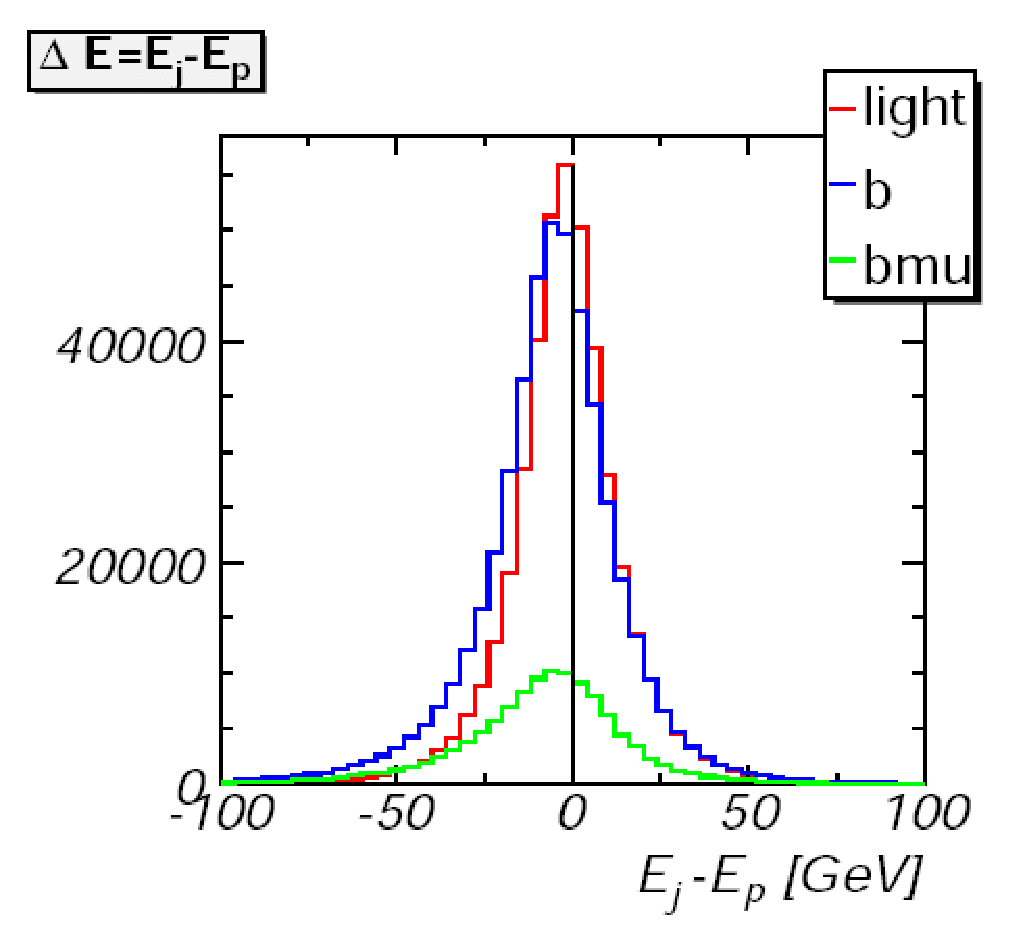
\includegraphics[width=0.4\textwidth]{figures/transfer/tfs}
\vspace{-0.1in}
\begin{minipage}{4in}
\caption[TF]{Energy difference between a jet and its matched parton
for three types of jets for all eta regions and all jet energies.}
\label{FlavorTF}
\end{minipage}
\end{figure}

The electron transfer function is described as a Gaussian distribution
with sigma dependent on the electron energy and
pseudorapidity~\cite{ElectronTF}. The muon transfer functions were
determined for muons with and without an SMT hit and are parametrized
as a function of $1/p_{T}$. The functions used in this analysis are
again the same as the ones used in the top mass
analysis~\cite{MuonTF,MuonTF2}.

\item $\Theta_{\rm{Parton}}(\vec{y})$ represents the parton level
cuts applied in order to avoid singularities in the matrix element
evaluation. These cuts are looser than the corresponding cuts at the
reconstructed level. All cross sections were calculated with the
following parton level cuts:

\begin{itemize}
\item Parton isolation: $\Delta$R($q_{i}$,$q_{j})>0.5$
\item Minimum parton $P_T$: $P_{T}(q_i)>6$ GeV
\item Maximum parton pseudorapidity: $|\eta(q_i)|<3.5$
\item No cuts applied to the lepton or neutrino
\end{itemize}

\item $\int d\vec{y}dq_{1}dq_{2}$ is an integration over the matrix
element phase space. The matrix element phase space for two parton
final state events is defined by the 14 independent spatial degrees of
freedom for the lepton, neutrino, and two partons as shown in
Eq.~\ref{dy}
\begin{equation}
\label{dy}
d\vec{y}_{2} = dq_{1}dq_{2}d|p|_{\ell}
d\Omega_{\ell}d|p|_{\nu}
d\Omega_{\nu}d|p|_{q1}
d\Omega_{q1}d|p|_{q2}
d\Omega_{q2}
\end{equation}

Events with three partons in the final state have 17 independent
degrees of freedom and has a phase space defined in Eq.~\ref{dy3jet}.
\begin{equation}
\label{dy3jet}
d\vec{y}_{3} = dq_{1}dq_{2}d|p|_{\ell}
d\Omega_{\ell}d|p|_{\nu}
d\Omega_{\nu}d|p|_{q1}
d\Omega_{q1}d|p|_{q2}
d\Omega_{q2}d|p|_{q3}
d\Omega_{q3}
\end{equation}

Four (six) degrees of freedom are removed from the integration for two
(three) parton event by assuming equal angles for partons and
jets. This approximation has been verified in Monte Carlo. Two more
degrees of freedom are removed by assuming well measured lepton
angles. Four more degrees of freedom are removed from the integration
by energy-momentum conservation, leaving four integration
variables. The final integration phase space is then transformed to
suit the matrix element being integrated. $W$+jets matrix element
integrations use the phase space defined in Eqs.~\ref{wjets_int} and
single top matrix element integrations use the phase space in
Eq.~\ref{st_int}. The phase space for events with three jets is shown
in Eq.~\ref{wjets_int_3jet} and~\ref{st_int_3jet}.
\begin{equation}
\label{wjets_int}
d\vec{y}_{\rm{W+jets - 2jets}}
= dr_{W}d|p_{q1}|d|p_{q2}|dp^{system}_{z}
\end{equation}
\begin{equation}
\label{st_int}
d\vec{y}_{\rm{single top - 2jets}} = dr_{\rm{top}}
dr_{W}d|p_{q2}|dp^{system}_{z}
\end{equation}
\begin{equation}
\label{wjets_int_3jet}
d\vec{y}_{\rm{W+jets - 3jets}}
= dr_{W}d|p_{q1}|d|p_{q2}|d|p_{q3}|dp^{system}_{z}
\end{equation}
\begin{equation}
\label{st_int_3jet}
d\vec{y}_{\rm{single top - 3jets}}
= dr_{\rm{top}}dr_{W}d|p_{q2}|d|p_{q3}|dp^{system}_{z}
\end{equation}
\noindent 
where $dr_{W}$ and $dr_{\rm{top}}$ are used to uniformly sample a Breit-Wigner distribution from the square of the
invariant mass distribution for $W$~boson and top quark production,
respectively. This choice of sampling minimizes integration time because the
matrix elements for these processes are negligable in regions where the invariant
mass of the lepton and neutrino is far from the $W$ mass and similarly for top
events where the mass of the lepton, neutrino, and $b$-quark is far from the top
mass. More information regarding the choice of variables and
the multidimensional integration can be found in
Appendix~\ref{full}. The multidimensional integrals were calculated
using the GNU~\cite{GNU} Scientific Library's version of the VEGAS
Monte Carlo integration technique~\cite{Lepage:1980dq}.

\end{itemize}

\subsubsection{Matrix Element Processes}

For events with exactly two jets, we consider a total of five matrix
elements for $2{\rar}4$ processes (top quark and $W$ bosons are
treated off-shell): s-channel single top ($ud{\rar}tb$), t-channel
single top ($ub{\rar}td$), $Wbb$ production ($ud{\rar}Wb\bar{b}$),
$Wcg$ production ($sg{\rar}Wcg$), and $Wgg$ production
($ud{\rar}Wgg$). ``tqb'' is used sometimes when referring to t-channel
events because the main diagram that describes these events is the
2$\rar$5 diagram with ``tqb'' in the final state. This analysis uses a
2$\rar$4 diagram with ``tq'' as the final state, as seen in
Fig~\ref{2jets}, because events with two jets require at most two
quarks or gluons in the final state. The three $W$+jets matrix
elements were chosen by running the Madgraph Monte Carlo generator and
selecting those processes which gave the largest cross section after
an overall $b$-tagging efficiency was applied. The leading order
diagrams for these channels (displayed as $2{\rar}3$ processes for
simplicity) are shown in Fig.~\ref{2jets}.

For events with three jets, we consider a total of three matrix
elements: s-channel single top ($ud{\rar}tbg$), t-channel single top
($ug{\rar}tbd$), and $Wbb$ production ($ud{\rar}Wb\bar{b}g$). The
number of $W$+jets matrix elements considered has been limited due to
the significant time required to compute the differential cross
section in Eq.~\ref{dsigma}. As will be discussed in
Section~\ref{disc-def}, this can only result in a reduced sensitivity
but does not affect the validity of the analysis. The leading order
diagrams for these channels (displayed as $2{\rar}3,4$ processes for
simplicity) are shown in Fig.~\ref{3jets}.

\clearpage

\begin{figure}[!h!tbp]
\includegraphics[width=0.27\textwidth]{figures/feynman/tb}
\hspace{0.2in}
\includegraphics[width=0.27\textwidth]{figures/feynman/tq}\\
\includegraphics[width=0.27\textwidth]{figures/feynman/wbb}
\hspace{0.2in}
\includegraphics[width=0.27\textwidth]{figures/feynman/wcg}
\hspace{0.2in}
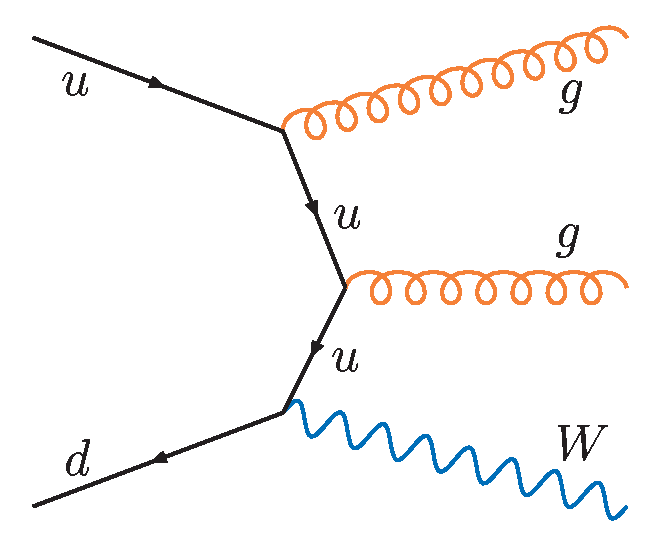
\includegraphics[width=0.27\textwidth]{figures/feynman/wgg}
\caption[2jets]{Representative Feynman diagrams corresponding to 
the leading-order matrix elements used for event probability
calculation for events with exactly two jets. Upper row, signals:
$ud{\rar}tb$, $ub{\rar}td$; lower row, backgrounds: $ud{\rar}Wbb$,
$sg{\rar}Wcg$, $ud{\rar}Wgg$.}
\label{2jets}
\end{figure}

\begin{figure}[!h!tbp]
\includegraphics[width=0.24\textwidth]{figures/feynman/tbg}
\hspace{0.2in}
\includegraphics[width=0.24\textwidth]{figures/feynman/tqb}
\hspace{0.2in}
\includegraphics[width=0.24\textwidth]{figures/feynman/wbbg}
\caption[3jets]{Representative Feynman diagrams corresponding to 
the leading-order matrix elements used for event probability
calculation for events with exactly three jets. Left two plots:
signals, $ud{\rar}tbg$, $ug{\rar}tbd$; right plot:
background,$ud{\rar}Wbbg$.}
\label{3jets}
\end{figure}

\subsubsection{Cross Section}

The event probability density function defined in Eq.~\ref{px}
requires a normalization constant to retain the probability density
interpretation. The normalization constant $\sigma$ is defined as the
detector level phase space integration $\int d\vec{x}$ of the
differential cross section defined in Eq.~\ref{dsigma}.
\begin{equation}
\label{cross}
\sigma = \sum_{i,j} \int d\vec{x}d\vec{y}
\left[ \pderiv{\sigma_{i,j}(\vec{y})}{\vec{y}}
\times W(\vec{x},\vec{y})
\times \Theta_{\rm{cuts}}(\vec{x})
\right]
\end{equation}
\noindent Because all the events for which the probability density
will be computed have had selection cuts applied, it is necessary to
consider this in the calculation of the cross section. The term
$\Theta_{\rm{cuts}}(\vec{x})$ is included in the calculation to
simulate the selection cuts. All cross sections were calculated with
the following selection cuts:

\begin{myitemize}
\item Lepton $P_{T}$ $>$ 15 GeV
\item Electron (muon) $|\eta|$ $<$ 1.1(2.0)
\item Missing $E_{T}$ $>$ 15 GeV
\item Leading jet $P_{T}$ $>$ 25 GeV
\item Leading jet $|\eta|$ $<$ 2.5
\item Second jet $P_{T}$ $>$ 20 GeV
\item Second jet $|\eta|$ $<$ 3.5
\item Third jet $P_{T}$ $>$ 20 GeV (if three-jet event)
\item Third jet $|\eta|$ $<$ 3.5 (if three-jet event)
\end{myitemize}

The selection cuts shown above are slighty different from the
canonical single top cuts. These cuts are included in the
normalization calculation to approximate the relative acceptance
difference between signal and background events. The cross sections
computed for each signal and background process for two- and three-jet
events are summarized in Table~\ref{cross-sections}. In all instances,
the statistical uncertainty from the Monte Carlo integration is below
$1\%$.

\begin{table}[!h!tbp]
\begin{center}
\begin{minipage}{5.5 in}
\begin{ruledtabular}
\begin{tabular}{l||cccccccc}
\multicolumn{9}{c}
{\underline{Cross Section $\times$ Branching Fraction [fb]}}
\vspace{0.05in} \\
            & \multicolumn{4}{c}{2-jet events}
            & \multicolumn{4}{c}{3-jet events} \\
            & \multicolumn{2}{c}{1 tag}
            & \multicolumn{2}{c}{2 tags}
            & \multicolumn{2}{c}{1 tag}
            & \multicolumn{2}{c}{2 tags}\\
            & Electron &   Muon   & Electron &   Muon
            & Electron &   Muon   & Electron &   Muon   \\
\hline
Signals     &    &     &     &    &    &     &    &     \\
~~$tb(g)$   &   8.07   &   10.4   &   6.90   &   8.90   
            &   6.02   &   7.64   &   5.22   &   6.66   \\
~~$tq(b)$   &  19.6    &   26.8   &   0.27   &   0.38   
            &   6.34   &    8.56  &   5.40   &   7.40   \\
Backgrounds &    &     &     &    &    &     &    &     \\
~~$Wbb(g)$  &  29.5    &   41.9   &  24.6    &  34.7    
            &   6.34   &   8.56   &   5.40   &   7.40   \\
~~$Wcg$     &  36.4    &   54.0   &   0.33   &   0.61   & & & & \\
~~$Wgg$     &  52.3    &   74.5   &   0.33   &   0.47   & & & &  
\end{tabular}
\end{ruledtabular}
\vspace{-0.1 in}
\caption[xsecs]{Cross section times branching fraction for each
analysis channel.}
\label{cross-sections}
\end{minipage}
\end{center}
\end{table}


\subsubsection{Treatment of Combinatorial Background}

The event probability density shown in Eq.~\ref{px} assumes a known
assignment between a jet and parton from the matrix element. In
practice, this assignment is not a-priori known and we must sum over
all possible assignments. In general, the event differential cross
section is modified as shown in Eq.~\ref{pxcomb}:
\begin{eqnarray}
\label{pxcomb}
d\sigma(\ell, j_1, j_2)
&=& \alpha_{j_1 {\rar} p_1} \alpha_{j_2 {\rar} p_2}
    d\sigma(\ell, j_1 {\rar} p_1, j_2 {\rar} p_2) + \nonumber \\
&+& \alpha_{j_2 {\rar} p_1} \alpha_{j_1 {\rar} p_2}
    d\sigma(\ell, j_2 {\rar} p_1, j_1 {\rar} p_2) 
\end{eqnarray}
\noindent where the $\alpha$ parameters relate to the probability of
the jet-parton match. If there is no a-priori knowledge of the correct
assignment, these quantities can be made equal. Thereby no preference
is given to either assignment.

This analysis uses information from the neural network
$b$~tagger~\cite{NNbtag} to weight the different jet-parton
combinations depending on whether a given jet is tagged or not and
which parton flavor is being assigned to it when summing over the
combinatorial background (see Eq.~\ref{pxcomb}). Therefore the
$\alpha$ weights are related to the jet tag-rate functions for the
different hypothesized jet flavors ($b$, $c$ and light), as shown in
Table~\ref{jp}. The different jet tag-rate functions for each flavor
have been provided by the B-ID group parametrized in terms of jet
$P_T$ and $\eta$: $\varepsilon_{\rm flavor}(j)=\varepsilon_{\rm
flavor}(P_T(j),\eta(j))$.

\begin{table}[!h!tbp]
\begin{center}
\begin{minipage}{3 in}
\begin{ruledtabular}
\begin{tabular}{c||cc}
\multicolumn{3}{c}
{\underline{Jet-Parton Matching Weight Factors}}\vspace{0.05in} \\
Parton flavor  &     $b$ tagged    &      Not tagged       \\
\hline
$b$            & $\varepsilon_{b}$ &  $1-\varepsilon_{b}$  \\
$c$            & $\varepsilon_{c}$ &  $1-\varepsilon_{c}$  \\
light          & $\varepsilon_{l}$ &  $1-\varepsilon_{l}$
\end{tabular}
\end{ruledtabular}
\vspace{-0.1 in}
\caption[jp]{Weights for the event differential cross section
depending on the $b$-tagging status of the jet and jet-parton
assignment.}
\label{jp}
\end{minipage}
\end{center}
\end{table}

For example, let us assume we have a given two-jet event with $j_1$
tagged and $j_2$ not tagged, and we are trying to evaluate the
probability density function for the $Wcg$ hypothesis, summing over
the two possible jet-parton assignments. In this case, the
differential cross section would be given by:
\begin{eqnarray}
\label{pxcomb_wcg}
d\sigma_{Wcg}(\ell, j_1, j_2)
&=& \varepsilon_{c}(j_1)(1-\varepsilon_{l}(j_2))
d\sigma_{Wcg}(\ell, j_1 {\rar} c, j_2 {\rar} g) + \nonumber \\ 
&+& \varepsilon_{l}(j_2))(1-\varepsilon_{c}(j_1))
d\sigma_{Wcg}(\ell, j_2 {\rar} c, j_1 {\rar} g).
\end{eqnarray}

This differential cross section must then be integrated over the
reconstructed lepton and jets four-momenta in order to compute the
event probability density function.

\subsection{Single Top Discriminant}

\subsubsection{Discriminant Definition}
\label{disc-def}

As discussed in Section~\ref{method-overview}, the signal and
background probability density functions are used to build an event
discriminant, defined in Eq.~\ref{disc2}. In particular, it is
possible to define discriminants specific to each of the single
top production modes, as well as inclusive for single top production, 
assuming the SM ratio of $s$- and $t$-channel cross sections.

The channel-specific discriminants are defined as:
\begin{equation}
D_{tb(tqb)}(\vec{x})
= \frac{P_{tb(tqb)}(\vec{x})}{P_{tb(tqb)}(\vec{x}) + P_{B}(\vec{x})}.
\label{disc1d}
\end{equation}
\noindent where $tqb$ here generically refers to the $t$-channel
process, whether based on the $tq$ matrix elements (two-jet events) or
the $tqb$ matrix elements (three-jet events).

%
% AJ 11/18/2006
% Comment this out since we won't be showing yet results from the
% tb+tqb discriminant
%
%The inclusive $tb$+$tqb$ discriminant is defined as:
%\begin{equation}
%D_{tb+tqb}(\vec{x})
%= \frac{\rho_{tb}P_{tb}(\vec{x})+(1-\rho_{tb})P_{tqb}(\vec{x})}
%{\rho_{tb}P_{tb}(\vec{x})+(1-\rho_{tb})P_{tqb}(\vec{x}) + P_{B}
%(\vec{x})},
%\label{disc1d_tbtqb}
%\end{equation}
%\noindent where $\rho_{tb}$ represents the expected 
%fraction of signal events from $s$-channel production after
%selection, which is
%computed for the different analysis channels and assuming the SM
%prediction
%of $\sigma_{tb}/\sigma_{tqb}=0.44$ (see Table~\ref{rhotb}).
%
%\vspace{0.05in}
%\begin{table}[!h!tbp]
%\begin{center}
%\begin{minipage}{3 in}
%\begin{ruledtabular}
%\begin{tabular}{l||cccc}
%\multicolumn{5}{c}
%{\hspace{0.5in}\underline{Expected $tb$ Fraction}}
%\vspace{0.1in} \\
%           & \multicolumn{2}{c}{1 tag} & \multicolumn{2}{c}{2 tags}\\
%           & Electron &   Muon   & Electron &   Muon   \\
%\hline
%2jet  &  {\color{red} X.XX}  &{  \color{red} X.XX}  
%5&  {\color{red} X.XX}  &  {\color{red} X.XX}  \\   
%3jet  &  {\color{red} X.XX}  &{  \color{red} X.XX}  
%&  {\color{red} X.XX}  &  {\color{red} X.XX}  \\    
%\end{tabular}
%\end{ruledtabular}
%\vspace{-0.1 in}
%\caption[rhotb]{Expected $tb$ fraction in selected single top
%events.}
%\label{rhotb}
%\end{minipage}
%\end{center}
%\end{table}

For two-jet events, the background probability density function
$P_B(\vec{x})$ is given by:
\begin{equation}
P_{B}(\vec{x})= C_{Wbb}P_{Wbb}(\vec{x})
              + C_{Wcg}P_{Wcg}(\vec{x})
              + C_{Wgg}P_{Wgg}(\vec{x}),
\label{probb}
\end{equation}
\noindent where $C_{Wbb}$, $C_{Wcg}$, and $C_{Wgg}$ are, in
principle, the relative fractions of each background in the
data. However, as discussed below, these background fractions are
optimized for the analysis.

The background fractions for the two-jet discriminant were found by a
grid search of each point ($C_{Wbb}$, $C_{Wcg}$, $C_{Wgg}$) and
calculating the expected Bayes ratio defined as the maximum of the
two-dimensional posterior divided by the value of the posterior at
zero signal cross section. This procedure was used by each analysis in
the single top group to optimize the final discriminant variable. The
values of the background fractions are summarized in Table~\ref{frac}.

\begin{table}[!h!tbp]
\begin{center}
\begin{minipage}{3 in}
\begin{ruledtabular}
\begin{tabular}{l||cccc}
\multicolumn{5}{c}
{\hspace{0.5in}\underline{Optimized Background Fractions}}
\vspace{0.1in} \\
           & \multicolumn{2}{c}{1 tag} & \multicolumn{2}{c}{2 tags}\\
           & Electron &   Muon   & Electron &   Muon   \\
\hline
$C_{Wbb}$  &   0.20   &   0.40   &   0.67   &     1    \\
$C_{Wcg}$  &   0.40   &   0.40   &     0    &     0    \\
$C_{Wgg}$  &   0.40   &   0.20   &   0.33   &     0
\end{tabular}
\end{ruledtabular}
\vspace{-0.1 in}
\caption[frac]{Background fractions chosen for each analysis channel
in two-jet events.}
\label{frac}
\end{minipage}
\end{center}
\end{table}

For the three-jet analysis, the background probability density
function $P_B(\vec{x})$ is given by:
\begin{equation}
P_{B}(\vec{x})= P_{Wbbg}(\vec{x}),
\label{probb_3j}
\end{equation}
\noindent which represents a further step in simplification relative
to the two-jet analysis.

At this point, a remark is in order. As can be seen, the background
probability density function does not contain multijet or $t\bar{t}$
matrix elements. Even for the case of $W$+jets, some simplifications
are made regarding which processes to consider and the relative
contributions of each of them to the total background probability
density. It should be stressed that the result of such approximations
can only be reduced discrimination. The background model still
contains all processes and the event discriminant is computed for all
of them to build the templates that will be compared to data.

\subsubsection{One-Dimensional Discriminants}

This section contains overlayed plots of the one-dimensional (1D) $tb$
and $tq$ discriminants for signal and background events. The events in
the plots come from the combined $e$,$\mu$ / 1,2 tags / 2,3 jets
channel. Figures~\ref{disc_wbb} and \ref{disc_wjets} show good
discrimination between signal and $W$+jets or multijets backgrounds.
However, the discrimination is poorer between signal and $\dilepton$
and $\lepjets$ events as shown in Fig.~\ref{disc_ttbar}. The lack of
discrimination power for $\ttbar$ events is due to the fact that the
current version of the analysis does not yet include a $\ttbar$
probability density function in the definition of the discriminant.
The $\ttbar$ matrix element takes much longer to integrate because
there are six partons in the final state while there are four in the
single top and $W$+jets matrix elements. Adding a $\ttbar$ matrix
element is envisioned as a future improvement for this analysis.

\begin{figure}[!h!tbp]
\includegraphics[width=0.40\textwidth]
{figures/performance/tb_Discriminant__schannel_wbb}
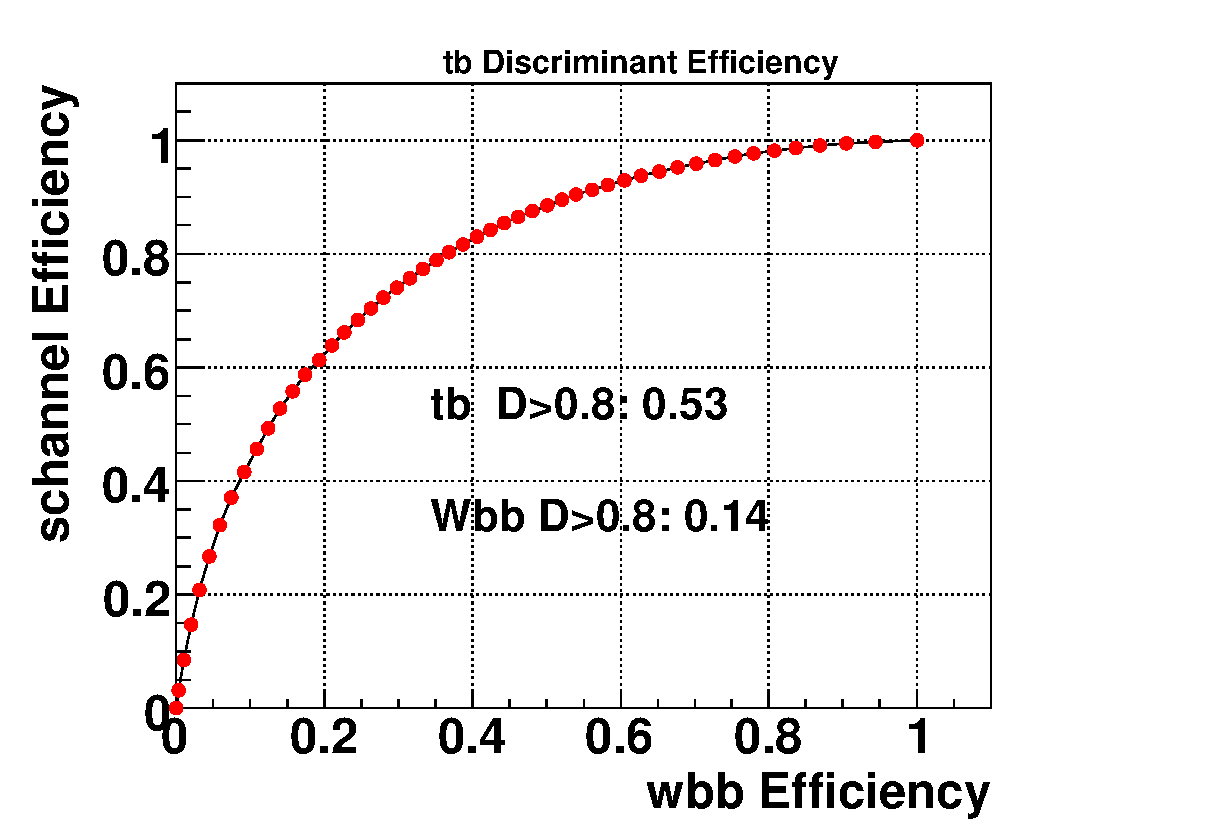
\includegraphics[width=0.40\textwidth]
{figures/performance/tb_Efficiency__schannel_wbb}
\includegraphics[width=0.40\textwidth]
{figures/performance/tb_Discriminant__schannel_wcc}
\includegraphics[width=0.40\textwidth]
{figures/performance/tb_Efficiency__schannel_wcc}
\includegraphics[width=0.40\textwidth]
{figures/performance/tq_Discriminant__tchannel_wbb}
\includegraphics[width=0.40\textwidth]
{figures/performance/tq_Efficiency__tchannel_wbb}
\includegraphics[width=0.40\textwidth]
{figures/performance/tq_Discriminant__tchannel_wcc}
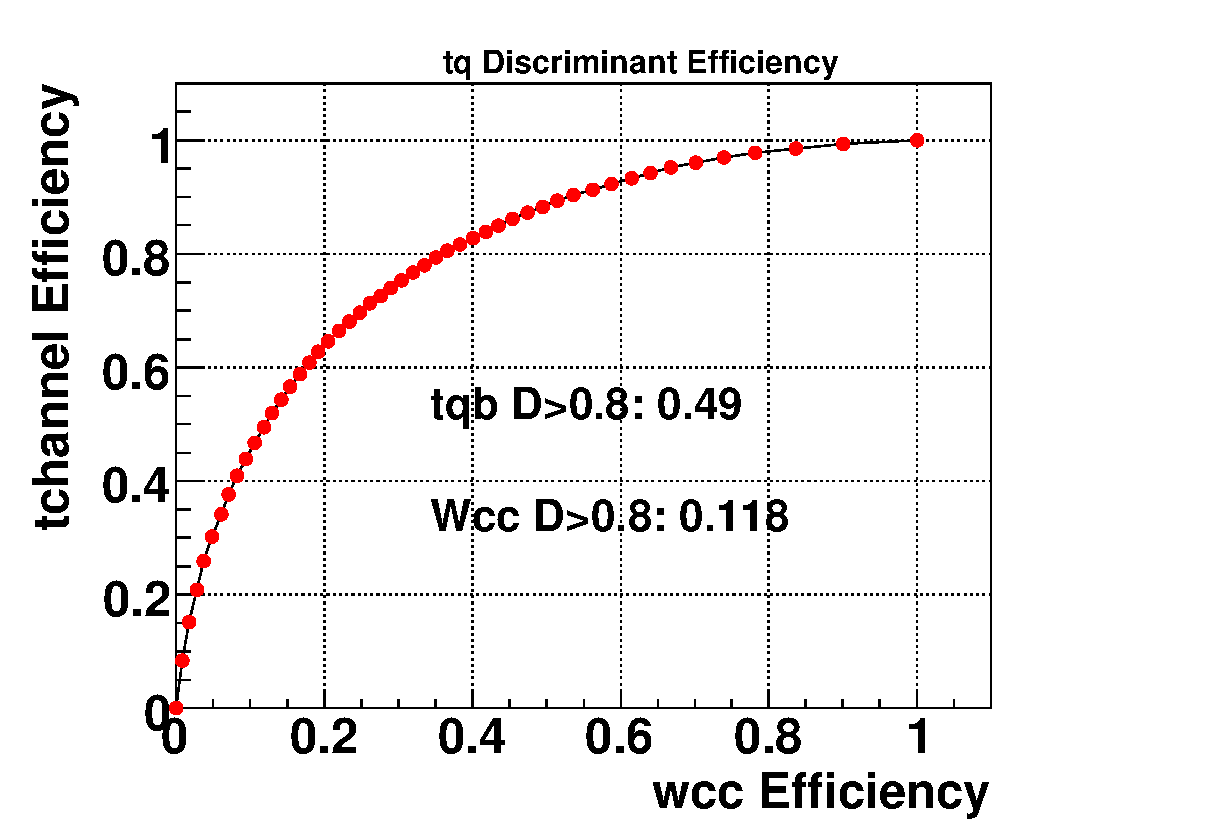
\includegraphics[width=0.40\textwidth]
{figures/performance/tq_Efficiency__tchannel_wcc}
\caption[discwbb]{Discriminant plots and efficiency curves for:
first row, $tb$ vs. $Wbb$, second row, $tb$ vs. $Wcc$, third row, $tq$
vs. $Wbb$, and fourth row, $tq$ vs. $Wcc$. The numbers in the
efficiency curves (right column) represent the fraction of signal or
background the remains after a discriminant cut of 0.8.}
\label{disc_wbb}
\end{figure}

\begin{figure}[!h!tbp]
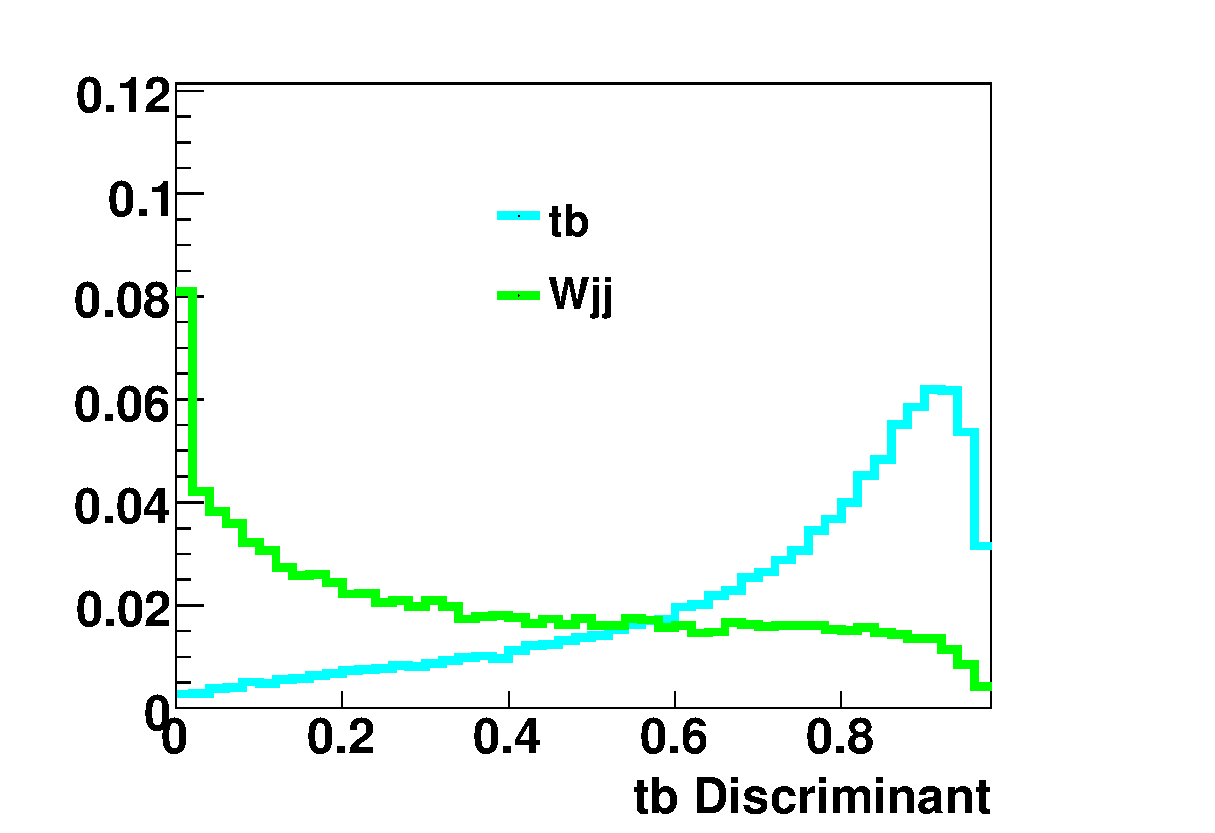
\includegraphics[width=0.40\textwidth]
{figures/performance/tb_Discriminant__schannel_wjj}
\includegraphics[width=0.40\textwidth]
{figures/performance/tb_Efficiency__schannel_wjj}
\includegraphics[width=0.40\textwidth]
{figures/performance/tb_Discriminant__schannel_qcd}
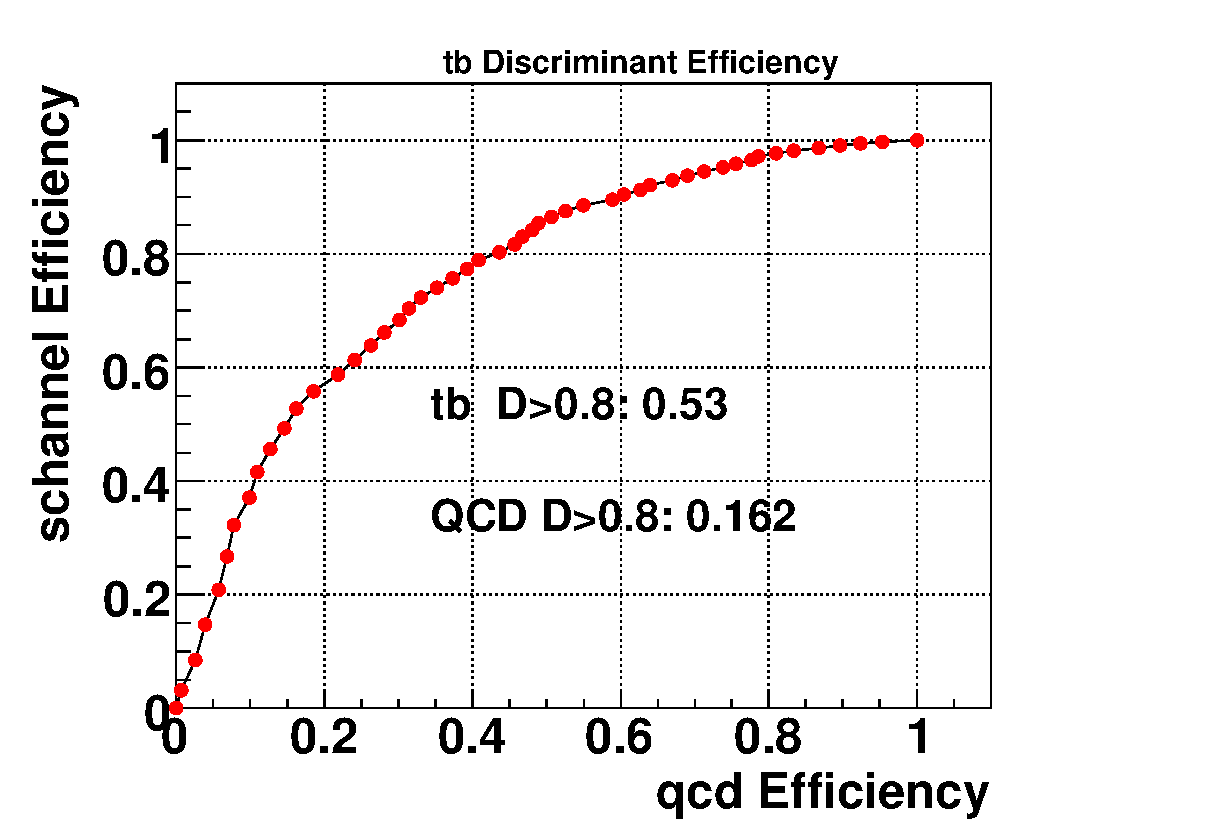
\includegraphics[width=0.40\textwidth]
{figures/performance/tb_Efficiency__schannel_qcd}
\includegraphics[width=0.40\textwidth]
{figures/performance/tq_Discriminant__tchannel_wjj}
\includegraphics[width=0.40\textwidth]
{figures/performance/tq_Efficiency__tchannel_wjj}
\includegraphics[width=0.40\textwidth]
{figures/performance/tq_Discriminant__tchannel_qcd}
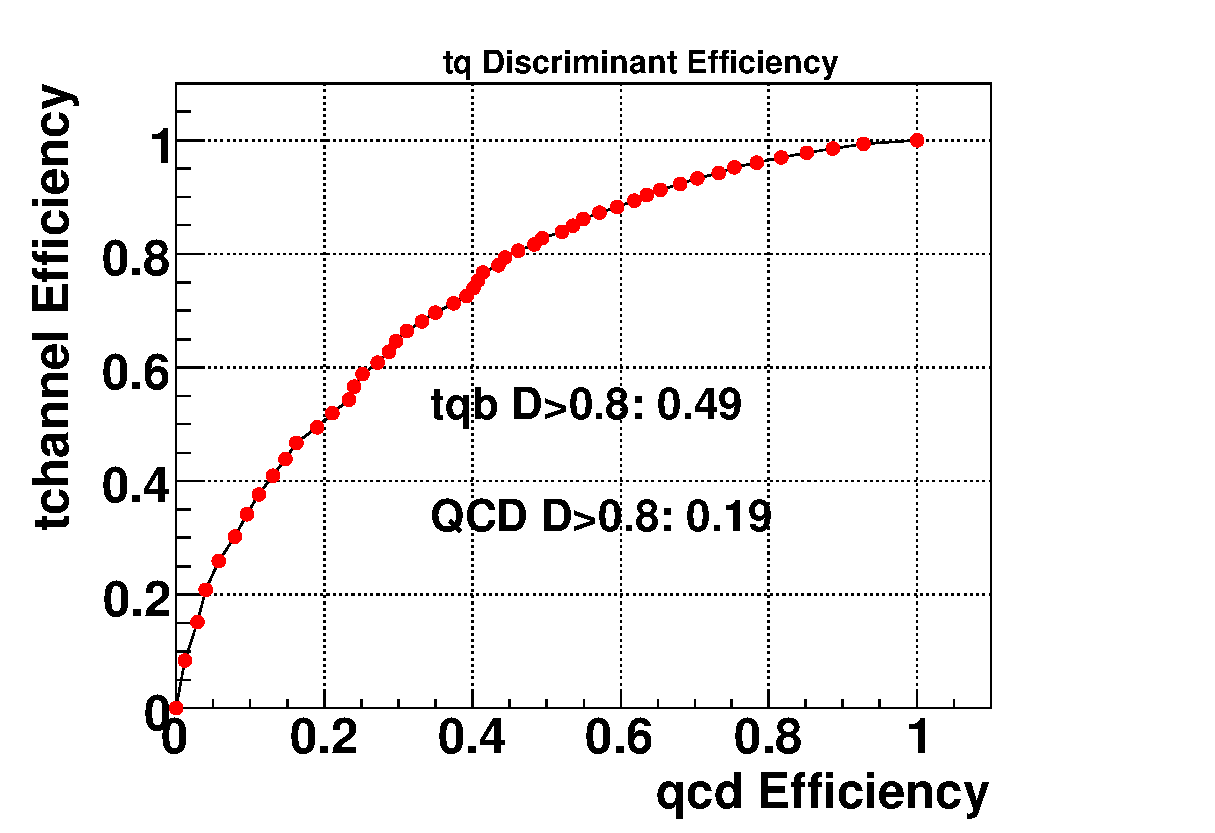
\includegraphics[width=0.40\textwidth]
{figures/performance/tq_Efficiency__tchannel_qcd}
\caption[discwjets]{Discriminant plots and efficiency curves for:
first row, $tb$ vs. $Wjj$, second row, $tb$ vs. multijets, third row,
$tq$ vs. $Wjj$, and fourth row, $tq$ vs. multijets. The numbers in the
efficiency curves (right column) represent the fraction of signal or
background the remains after a discriminant cut of 0.8.}
\label{disc_wjets}
\end{figure}

\begin{figure}[!h!tbp]
\includegraphics[width=0.40\textwidth]
{figures/performance/tb_Discriminant__schannel_dilepton}
\includegraphics[width=0.40\textwidth]
{figures/performance/tb_Efficiency__schannel_dilepton}
\includegraphics[width=0.40\textwidth]
{figures/performance/tb_Discriminant__schannel_lepjets}
\includegraphics[width=0.40\textwidth]
{figures/performance/tb_Efficiency__schannel_lepjets}
\includegraphics[width=0.40\textwidth]
{figures/performance/tq_Discriminant__tchannel_dilepton}
\includegraphics[width=0.40\textwidth]
{figures/performance/tq_Efficiency__tchannel_dilepton}
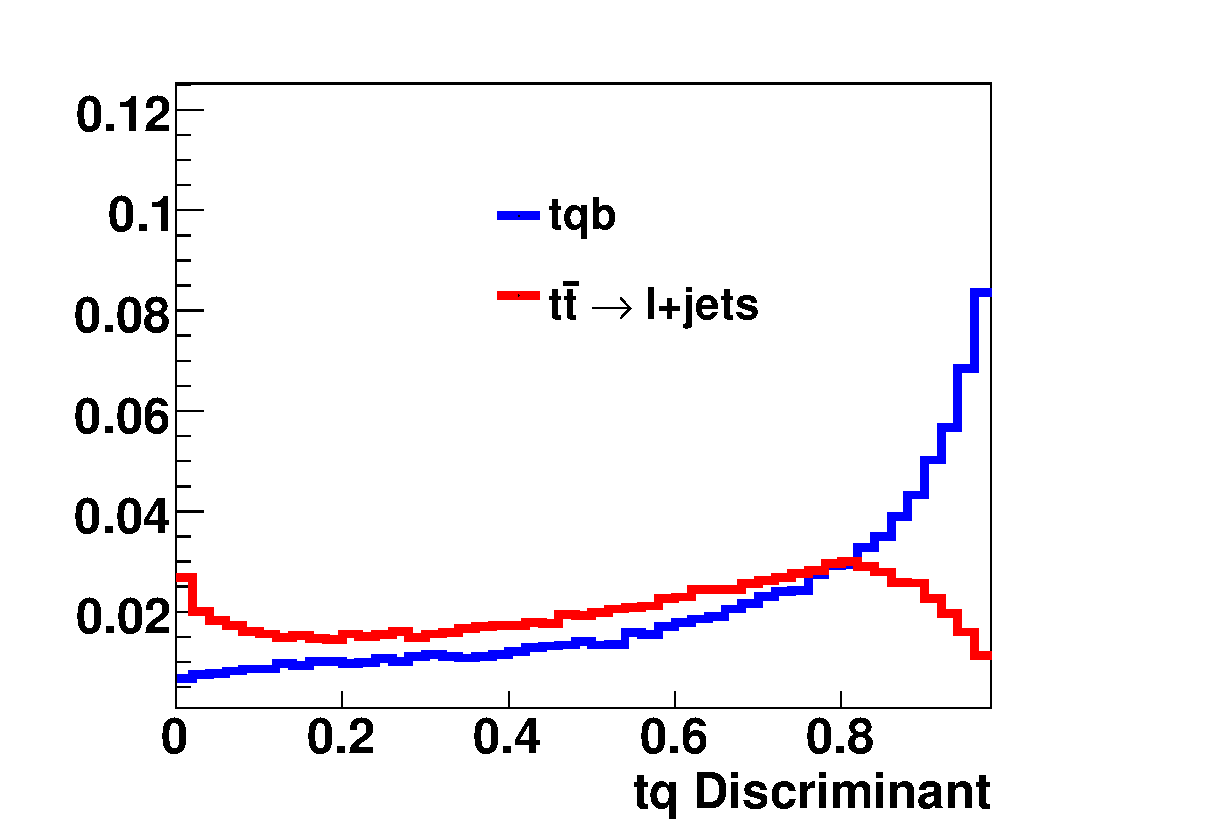
\includegraphics[width=0.40\textwidth]
{figures/performance/tq_Discriminant__tchannel_lepjets}
\includegraphics[width=0.40\textwidth]
{figures/performance/tq_Efficiency__tchannel_lepjets}
\caption[discttbar]{Discriminant plots and efficiency curves for:
first row, $tb$ vs. $\dilepton$, second row, $tb$ vs. $\lepjets$,
third row, $tq$ vs. $\dilepton$, and fourth row, $tq$
vs. $\lepjets$. The numbers in the efficiency curves (right column)
represent the fraction of signal or background the remains after a
discriminant cut of 0.8.}
\label{disc_ttbar}
\end{figure}

\subsubsection{Two-Dimensional Discriminants}

This analysis uses a two-dimensional (2D) discriminant computed from
the 1D $tb$ and $tq$ discriminants discussed in the previous
section. The 2D discriminant is more powerful than either 1D
projection because it selects events with both $tb$ and $tq$
characteristics, which helps to further reduce the $W$+jets and
$\ttbar$ background which may have either characteristic but not
necessarily both. 
%Furthermore, the simultaneous sensitivity to both
%production channels makes the 2D discriminant an essential tool to
%perform a model-independent search and/or cross section measurement,
%without having to make assumptions about e.g., the $tb$:$tq$ cross
%section ratio. 

Figures~\ref{wbbwccwjj} and \ref{qcdtt} show the 2D discriminants
for single top quark signals and for all the backgrounds. The
plots are normalized to unit volume.

\clearpage

\begin{figure}[!h!tbp]
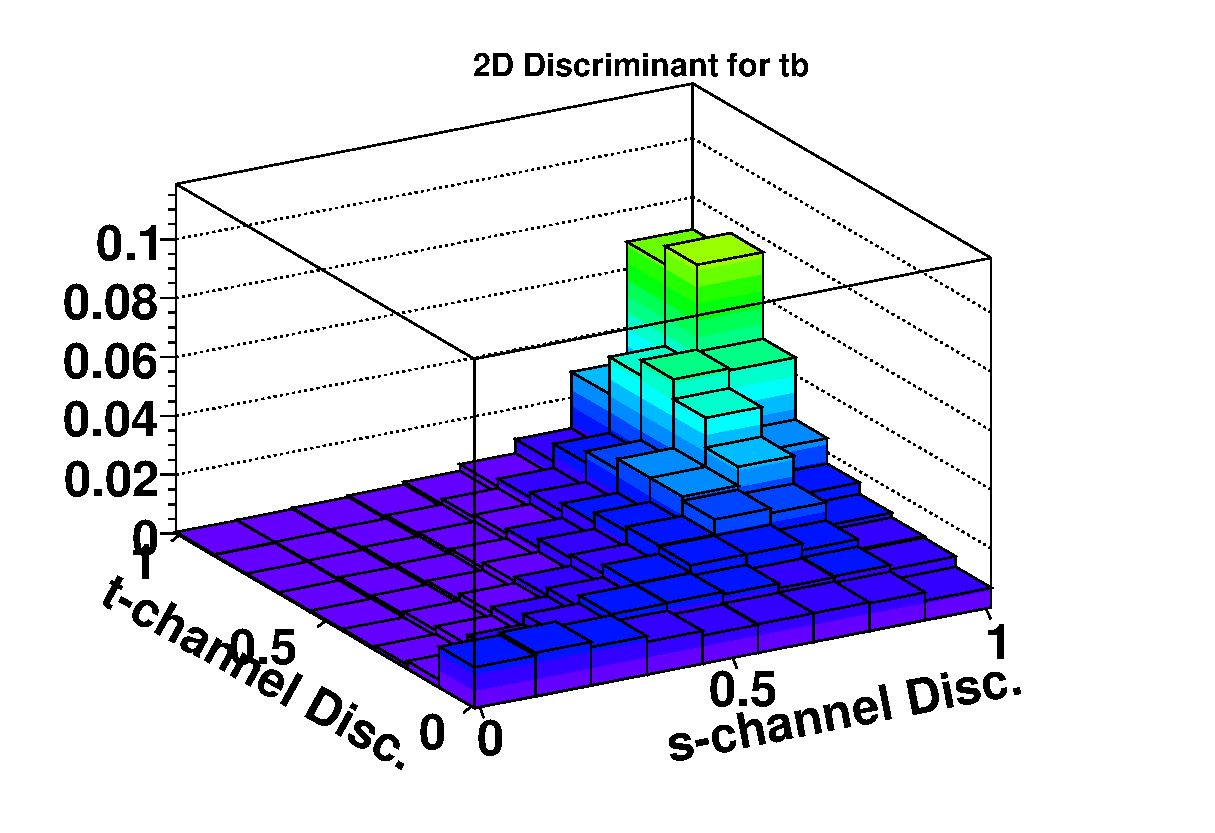
\includegraphics[width=0.32\textwidth]
{figures/performance/2D-Discriminant_schannel}
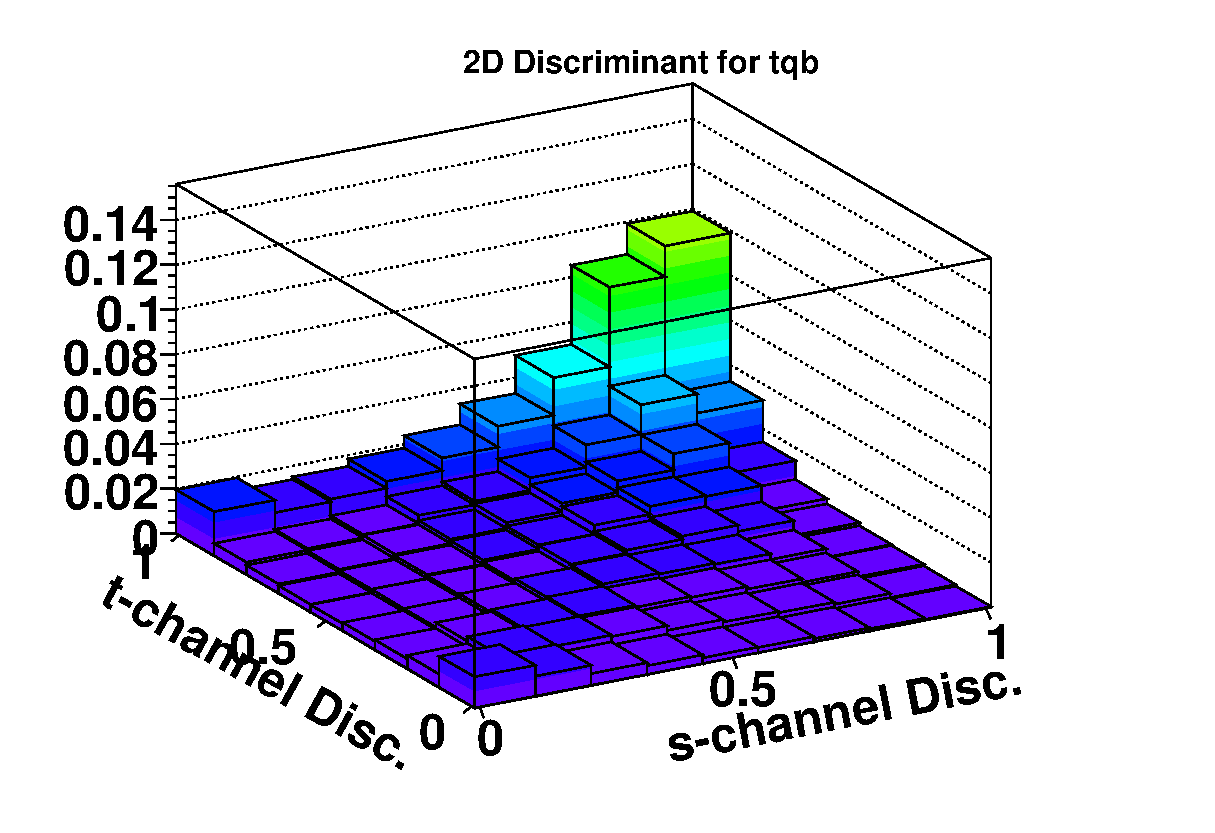
\includegraphics[width=0.32\textwidth]
{figures/performance/2D-Discriminant_tchannel}
\vspace{-0.1in}
\caption[tbtqwbbwcc]{2D-discriminant templates for: left, $tb$, and
right, $tqb$ Monte Carlo events.}
\label{tbtqb}
\end{figure}

\begin{figure}[!h!tbp]
\includegraphics[width=0.32\textwidth]
{figures/performance/2D-Discriminant_wbb}
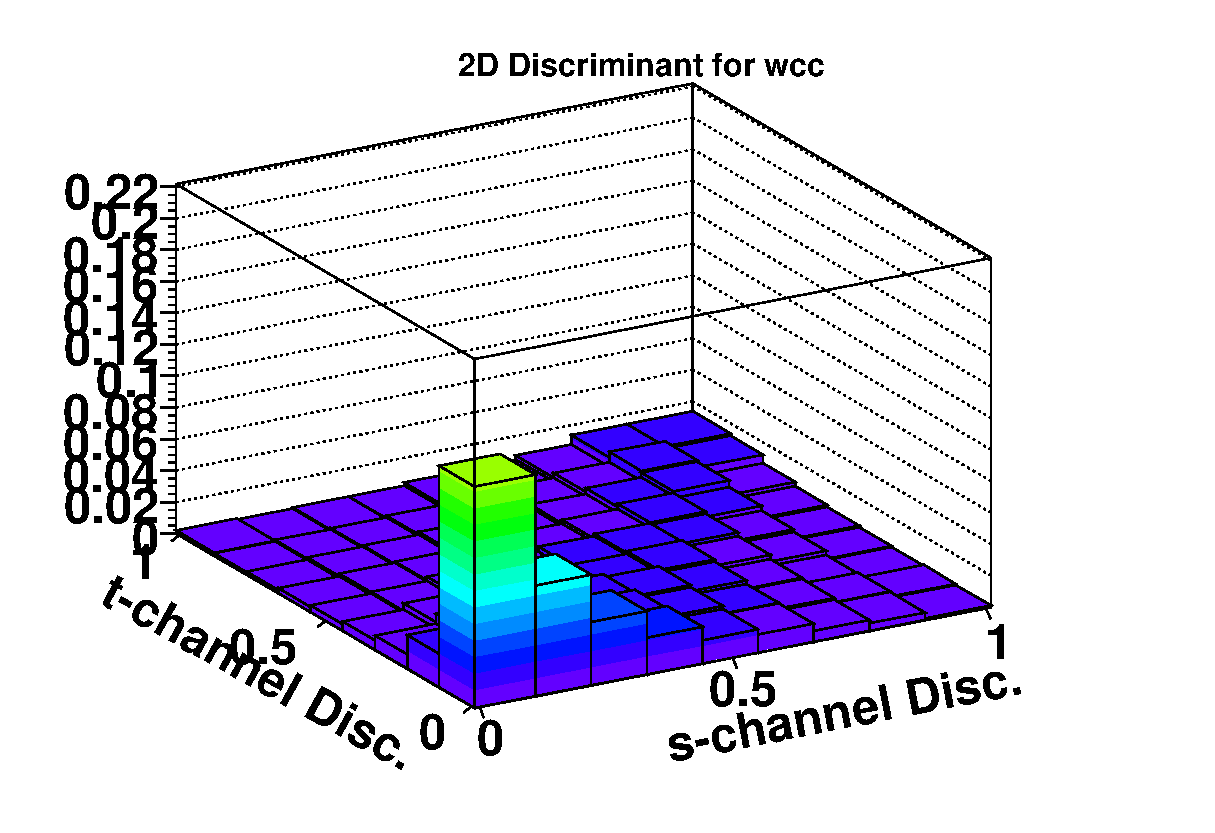
\includegraphics[width=0.32\textwidth]
{figures/performance/2D-Discriminant_wcc}
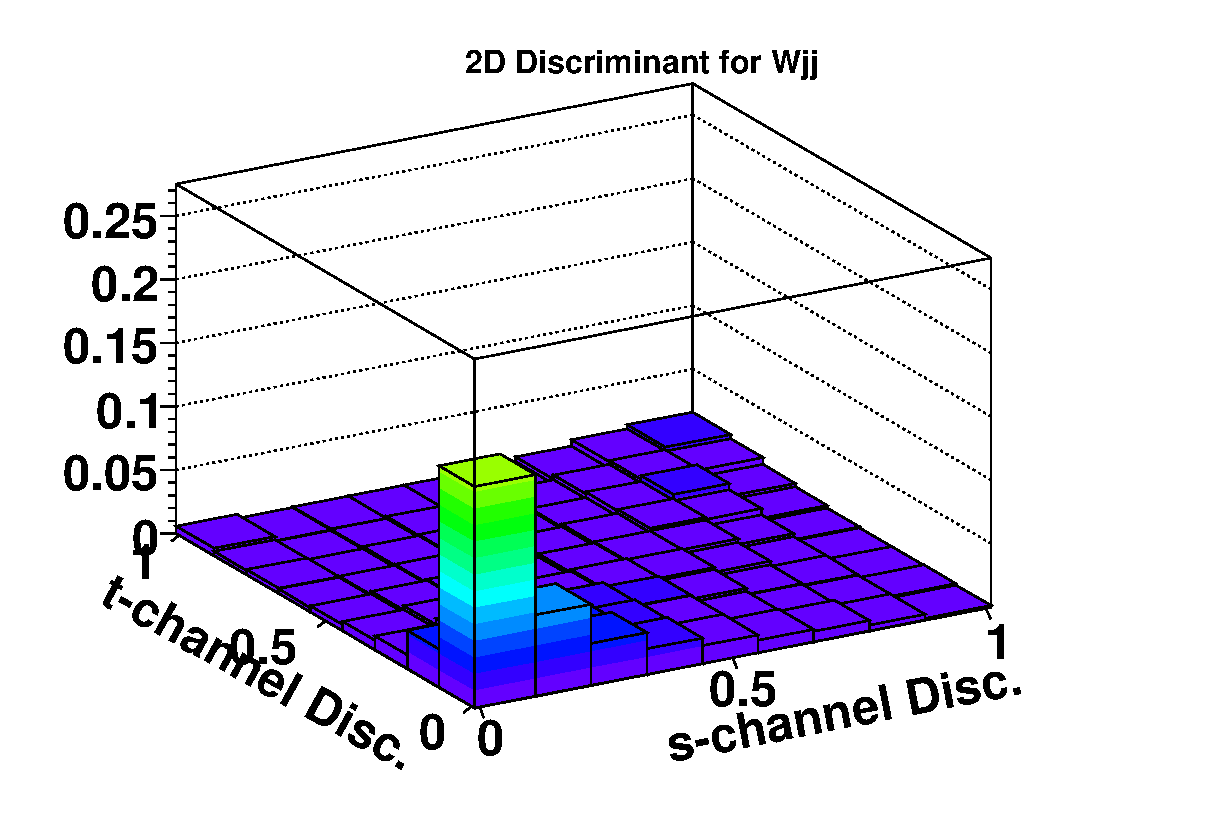
\includegraphics[width=0.32\textwidth]
{figures/performance/2D-Discriminant_wjj}
\vspace{-0.1in}
\caption[tbtqwbbwcc]{2D-discriminant templates for: left,
$Wbb$, middle, $Wcc$, and right, $Wjj$ Monte Carlo events.}
\label{wbbwccwjj}
\end{figure}

\begin{figure}[!h!tbp]
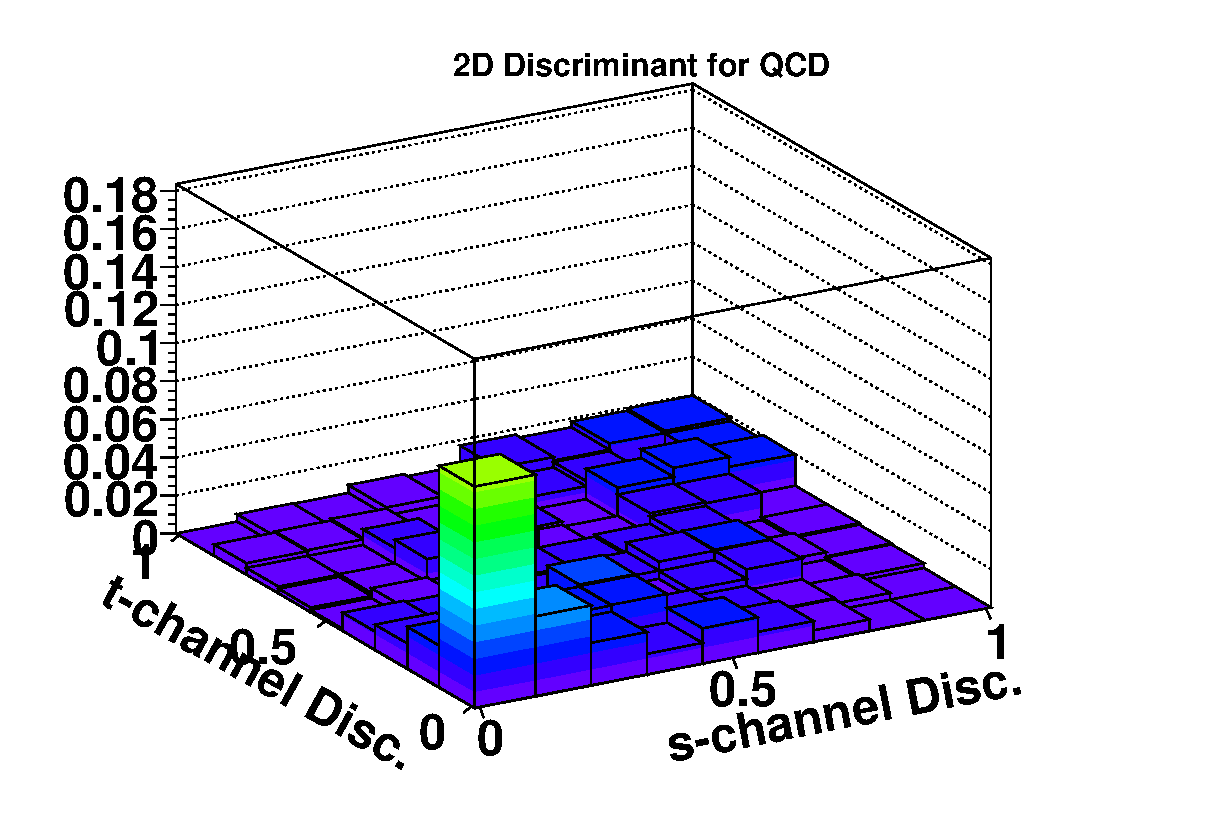
\includegraphics[width=0.32\textwidth]
{figures/performance/2D-Discriminant_qcd}
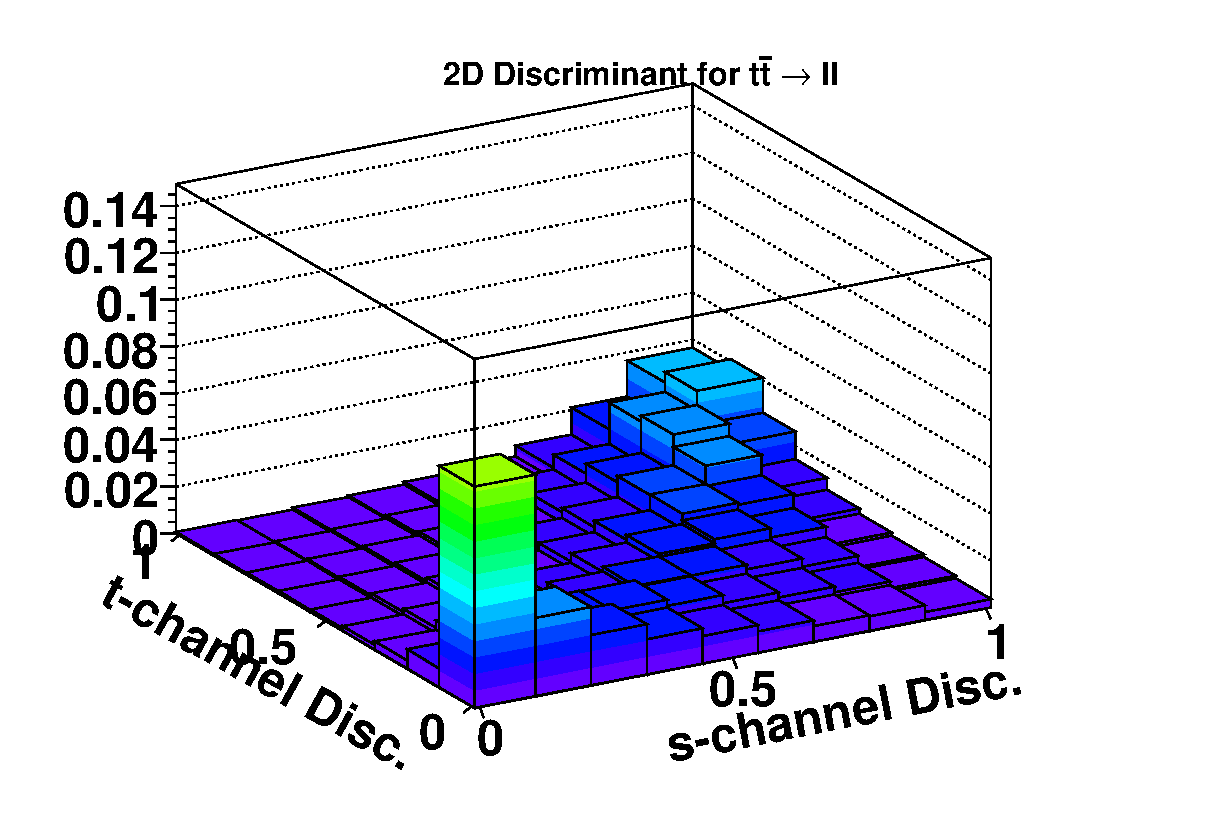
\includegraphics[width=0.32\textwidth]
{figures/performance/2D-Discriminant_dilepton}
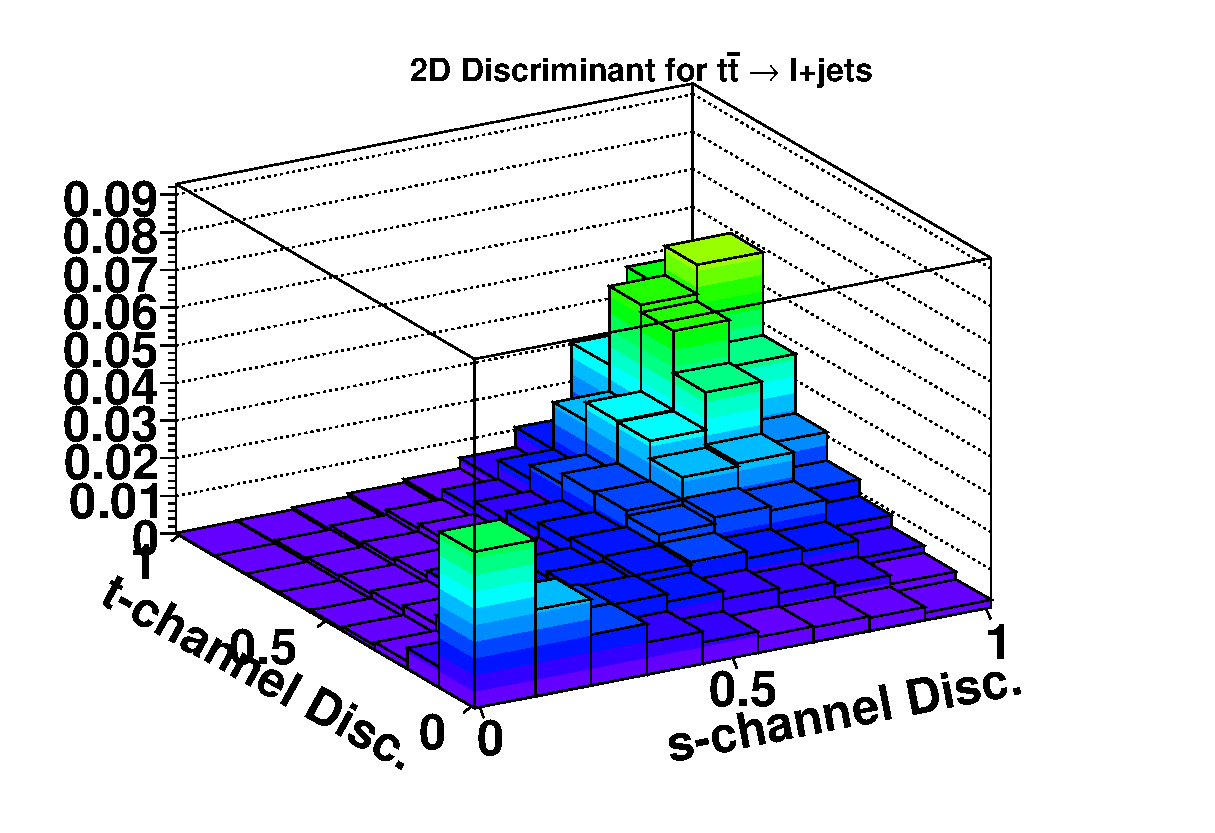
\includegraphics[width=0.32\textwidth]
{figures/performance/2D-Discriminant_lepjets}
\vspace{-0.1in}
\caption[wjjqcdtt]{2D-discriminant templates for: left,
multijets events, middle, $\dilepton$, and right, $\lepjets$ Monte
Carlo events.}
\label{qcdtt}
\end{figure}



\clearpage
%---------------------------------------------------------------------
\section{Cross-Check Samples}
\label{data-MC}

A crucial step in the single top search is to establish that the
background model is appropriate while minimizing looking into the
search region. For this purpose, two background-dominated control
samples are defined, and a comparison between the 1D discriminants in
data and the background model is performed.

These two control samples are selected by applying the standard event
selection, and requiring in addition $H_T<175$~GeV and $H_T>300$~GeV,
respectively. Two-jet events are largely dominated by $W$+jets
events, and thus it is the modeling of this background that is mainly
addressed by these cross checks. We refer to these control samples as
``soft $W$+jets'' and ``hard $W$+jets'' respectively. In the case of
three-jet events, the ``hard $W$+jets'' sample also contains a
significant fraction of $\ttbar$.

The ``soft $W$+jets'' sample selects low momentum $W$+jets and
multijets events and almost no top-quark events.
Figures~\ref{wjets-cross-2jet} and \ref{wjets-cross-3jet} compare the
$tb$ and $tq$ discriminants between data and the background model for
events with two and three jets respectively. Good agreement is seen
between data and expectation.

The ``hard $W$+jets'' sample selects mainly $\ttbar$ and high momentum
$W$+jets events. Figures~\ref{ttbar-cross-2jet} and
\ref{ttbar-cross-3jet} compare the $tb$ and $tq$ discriminants between
data and the background model for events with two and three jets. Good
agreement is again found between data and expectation.

Most of the signal, and thus the problematic $W$+jets background, has
$H_T$ between these cuts. Therefore, by confirming that the observed
discriminant distribution is well reproduced by the background model
for the softest and hardest $W$+jets events, we gain confidence that
the $W$+jets background in the signal region is also well modeled.

\clearpage

\begin{figure}[!h!tbp]
\includegraphics[width=0.40\textwidth]
{figures/cross_check/combined/2jet/Wjets_tb_Discriminant}
\includegraphics[width=0.40\textwidth]
{figures/cross_check/combined/2jet/Wjets_tb_Discriminant_Zoom}
\includegraphics[width=0.40\textwidth]
{figures/cross_check/combined/2jet/Wjets_tq_Discriminant}
\includegraphics[width=0.40\textwidth]
{figures/cross_check/combined/2jet/Wjets_tq_Discriminant_Zoom}
\vspace{-0.1in}
\caption[wjetscross]{``Soft $W$+jets'' cross-check plots in two-jet
events for the $tb$ discriminant (upper row) and the $tq$ discriminant
(lower row). The left column shows the full discriminant region while
the right column shows the high discriminant region above 0.7.}
\label{wjets-cross-2jet}
\end{figure}

\begin{figure}[!h!tbp]
\includegraphics[width=0.40\textwidth]
{figures/cross_check/combined/3jet/Wjets_tb_Discriminant}
\includegraphics[width=0.40\textwidth]
{figures/cross_check/combined/3jet/Wjets_tb_Discriminant_Zoom}
\includegraphics[width=0.40\textwidth]
{figures/cross_check/combined/3jet/Wjets_tq_Discriminant}
\includegraphics[width=0.40\textwidth]
{figures/cross_check/combined/3jet/Wjets_tq_Discriminant_Zoom}
\vspace{-0.1in}
\caption[wjetscross]{``Soft $W$+jets'' cross-check plots in three-jet
events for the $tb$ discriminant (upper row) and the $tq$ discriminant
(lower row). The left column shows the full discriminant region while
the right column shows the high discriminant region above 0.7.}
\label{wjets-cross-3jet}
\end{figure}

\begin{figure}[!h!tbp]
\includegraphics[width=0.40\textwidth]
{figures/cross_check/combined/2jet/TTbar_tb_Discriminant}
\includegraphics[width=0.40\textwidth]
{figures/cross_check/combined/2jet/TTbar_tb_Discriminant_Zoom}
\includegraphics[width=0.40\textwidth]
{figures/cross_check/combined/2jet/TTbar_tq_Discriminant}
\includegraphics[width=0.40\textwidth]
{figures/cross_check/combined/2jet/TTbar_tq_Discriminant_Zoom}
\vspace{-0.1in}
\caption[ttbarcross]{``Hard $W$+jets'' cross-check plots in two-jet
events for the $tb$ discriminant (upper row) and the $tq$ discriminant
(lower row). The left column shows the full discriminant region while
the right column shows the high discriminant region above 0.7.}
\label{ttbar-cross-2jet}
\end{figure}

\begin{figure}[!h!tbp]
\includegraphics[width=0.40\textwidth]
{figures/cross_check/combined/3jet/TTbar_tb_Discriminant}
\includegraphics[width=0.40\textwidth]
{figures/cross_check/combined/3jet/TTbar_tb_Discriminant_Zoom}
\includegraphics[width=0.40\textwidth]
{figures/cross_check/combined/3jet/TTbar_tq_Discriminant}
\includegraphics[width=0.40\textwidth]
{figures/cross_check/combined/3jet/TTbar_tq_Discriminant_Zoom}
\vspace{-0.1in}
\caption[ttbarcross]{``Hard $W$+jets'' cross-check plots in three-jet
events for the $tb$ discriminant (upper row) and the $tq$ discriminant
(lower row). The left column shows the full discriminant region while
the right column shows the high discriminant region above 0.7.}
\label{ttbar-cross-3jet}
\end{figure}



\clearpage
%---------------------------------------------------------------------
\section{Ensemble Tests}
\label{sec:ensembles}

Several ensembles of pseudo-data events were produced from the
background model to test the performance of the analysis. These
ensembles include:
\vspace{-0.05in}
\begin{myenumerate}
\item 400 fake data samples with SM single top content
($\sigma_{tb+tqb}=2.86$~pb).
\item Four sets of 100 samples each (named A, B, C and D), with
unknown (to the analyzers) single top content, but with SM ratios
between the $tb$ and $tqb$ cross sections.
\item Two sets of 200 samples with the SM ratio between the $tb$ and
$tqb$ cross sections, and with a total single top cross section of
$\sigma_{tb+tqb}=4.5$~pb and $\sigma_{tb+tqb}=4.7$~pb.
% Uncomment once the final set of results and plots are done:
%\item 6 sets of 100 experiments with unknown total cross section and
%      unknown $tb$:$tqb$ ratio
\end{myenumerate}
\vspace{-0.05in}
The full analysis chain was run using each pseudo-dataset as if it
were the real dataset. The results are presented in the following
subsections.

\subsection{Ensemble Tests with SM Signal}
\label{ens_SM_sig}

Figure~\ref{SMens} shows the distribution of estimated cross sections
from one ensemble generated with the SM input signal cross sections
for the electron, muon, and e+$\mu$ channel. The ensemble contains 400
samples of both 2-jet and 3-jet events. The input cross section in
each case is 2.86~pb. The most probable value of the distribution is
2.75~pb while the mean is 3.18~pb.

\vspace{0.1in}
\begin{figure}[!h!tbp]
\includegraphics[width=0.40\textwidth]
{figures/ensembles/Ensembles_Electron}
\includegraphics[width=0.40\textwidth]
{figures/ensembles/Ensembles_Muon}
\includegraphics[width=0.40\textwidth]
{figures/ensembles/Ensembles}
\vspace{-0.1in}
\caption[SMens]{Results of standard model ensemble test for the
electron channel (upper left plot), the muon channel (upper right
plot), and electrons and muons combined (lower plot).}
\label{SMens}
\end{figure}

\clearpage

\subsection{Ensemble Tests with Non-SM Signal}
\label{ens_nonSM_sig}

Five more ensembles were generated with a non-SM $tb$+$tqb$ cross
section, but SM $tb$:$tqb$ cross section ratio ($\sigma_s/\sigma_t =
0.44$). The results are shown in Fig.~\ref{ensembles}.

\vspace{0.1in}
\begin{figure}[!h!tbp]
\includegraphics[width=0.40\textwidth]{figures/ensembles/EnsemblesA}
\includegraphics[width=0.40\textwidth]{figures/ensembles/Ensembles0sig1}
\includegraphics[width=0.40\textwidth]{figures/ensembles/EnsemblesC}
\includegraphics[width=0.40\textwidth]{figures/ensembles/EnsemblesD}
\includegraphics[width=0.40\textwidth]{figures/ensembles/Ensembles4.5.eps}
\includegraphics[width=0.40\textwidth]{figures/ensembles/Ensembles4.7.eps}
\vspace{-0.1in}
\caption{Results using the ensembles with non-SM cross section but
SM $tb$:$tqb$ ratio. The upper row contains ensembles A and B, the
middle row shows ensembles C and D, the bottom row shows the results
from two ensembles with input cross sections close to our measured
cross section of 4.6~pb.}
\label{ensembles}
\end{figure}

Our measured values of the cross sections taken from the means of the
ensembles are:
\vspace{-0.05in}
\begin{myitemize}
\item A: 3.00 $\times$ SM \hspace{0.2in}(true value = 2.76 $\times$ SM)
\item B: 0.20 $\times$ SM \hspace{0.2in}(true value = 0)
\item C: 0.86 $\times$ SM \hspace{0.2in}(true value = 0.70 $\times$ SM)
\item D: 2.38 $\times$ SM \hspace{0.2in}(true value = 2.06 $\times$ SM)
\end{myitemize} 

We show these measured cross sections versus the input values in
Fig.~\ref{calibration} as a calibration check. We fit a straight line
through points greater than 1~pb where it shows good agreement with
the measurements. Below that, the measurement is biased to produce a
value greater than input because the results are constrained to be
positive.

\clearpage

\vspace{0.1in}
\begin{figure}[!h!tbp]
\begin{center}
\includegraphics[width=0.65\textwidth]{figures/ensembles/ME_analysis}
\end{center}
\vspace{-0.1in}
\caption[calibration]{Measured signal cross section versus input
cross section in the ensemble tests. The ensemble response is obtained
from the mean of the distributions in Figs.~\ref{SMens} and
\ref{ensembles}.}
\label{calibration}
\end{figure}



\clearpage
%---------------------------------------------------------------------
\section{Expected Results}
\label{exp-performance}

In this section we present results regarding the expected performance
of the analysis. To obtain these results the number of observed events
has been set equal to the expected signal, according to the standard
model prediction, plus the expected background.

Figures.~\ref{exp-post-1d-2j} and \ref{exp-post-1d-3j} show the
resulting $tb$+$tqb$ posterior for the combined $e$+$\mu$ $\geq$~1
$b$-tag channel in two-jet and three-jet events.
Figure~\ref{exp-post-1d-allj} shows the $tb$+$tqb$ posterior for the
combination of all channels. The left figures correspond to the case
of only statistical uncertainties considered, whereas the right
figures also include systematic uncertainties.

\vspace{0.1in}
\begin{figure}[!h!tbp]
\includegraphics[width=0.37\textwidth]
{figures/posterior/nosys/expected_limit_TBTQ_LeptonsCombined_2Jet_TagsCombined}
\includegraphics[width=0.37\textwidth]
{figures/posterior/sys/expected_limit_TBTQ_LeptonsCombined_2Jet_TagsCombined}
\vspace{-0.1in}
\caption[exppost1d2j]{Expected 1D posterior plots for the combined
$e$+$\mu$ $\geq$~1 $b$-tag channel in two-jet events, with statistical
uncertainties only (left plot) and including also systematic
uncertainties (right plot).}
\label{exp-post-1d-2j}
\end{figure}

\vspace{0.1in}
\begin{figure}[!h!tbp]
\includegraphics[width=0.37\textwidth]
{figures/posterior/nosys/expected_limit_TBTQ_LeptonsCombined_3Jet_TagsCombined}
\includegraphics[width=0.37\textwidth]
{figures/posterior/sys/expected_limit_TBTQ_LeptonsCombined_3Jet_TagsCombined}
\vspace{-0.1in}
\caption[exppost1d3j]{Expected 1D posterior plots for the combined
$e$+$\mu$ $\geq$~1 $b$-tag channel in three-jet events, with
statistical uncertainties only (left plot) and including also
systematic uncertainties (right plot).}
\label{exp-post-1d-3j}
\end{figure}

\vspace{0.1in}
\begin{figure}[!h!tbp]
\includegraphics[width=0.37\textwidth]
{figures/posterior/nosys/expected_limit_TBTQ_LeptonsCombined_JetsCombined_TagsCombined}
\includegraphics[width=0.37\textwidth]
{figures/posterior/sys/expected_limit_TBTQ_LeptonsCombined_JetsCombined_TagsCombined}
\vspace{-0.1in}
\caption[exppost1dallj]{Expected 1D posterior plots for the
combination of all channels, with statistical uncertainties only (left
plot) and including also systematic uncertainties (right plot).}
\label{exp-post-1d-allj}
\end{figure}

\subsection{Expected Signal Significance}

We calculate the significance of the expected results using the
$tb$+$tqb$ posteriors presented in the previous section. The Bayes
ratio (see Appendix~10 in Ref.~\cite{general-note}) is defined as the
peak value of the posterior divided by the posterior at zero signal
cross section. The larger the Bayes ratio, the larger the expected
significance of the result. This measure has been used to optimize the
analysis in the individual channels.  Results are shown in
Table~\ref{bayes-ratio}.

\begin{table}[!h!tbp]
\begin{center}
\begin{minipage}{5in}
\begin{ruledtabular}
\begin{tabular}{l|cc|cc|cc|c}
  \multicolumn{8}{c}{\hspace{0.5in}\underline{Expected Bayes Ratios for the $tb$+$tqb$ Signal}}\vspace{0.1in}\\
& \multicolumn{2}{c|}{1,2tags + 2,3jets}& \multicolumn{2}{c|}{$e$,$\mu$ + 2,3jets}
& \multicolumn{2}{c|}{$e$,$\mu$ + 1,2tags}& All \\
                 &  $e$-chan & $\mu$-chan& 1 tag & 2 tags& 2 jets& 3 jets&channels\\
\hline
Statistics only  &  $8.1$  & $4.1$ & $17.8$ & $1.9$ & $15.9$ & $2.1$ & $33.3$     \\
With systematics &  $3.8$  & $2.6$ & $6.3$  & $1.4$ & $6.2$  & $1.3$ & $\mathbf{8.4}$     \\
\end{tabular}
\end{ruledtabular}
\vspace{-0.1in}
\caption[bayesratio]{Expected Bayes ratios, without and with
systematic uncertainties, for many combinations of analysis
channels. The best value from all channels combined, with
systematics, is shown in bold type.}
\label{bayes-ratio}
\end{minipage}
\end{center}
\end{table}

% AJ 11/18/2006  
% I'm commenting this out since this S/sqrt{B} would best be evaluated
% cutting on the s+t discriminant
%
%A third method is to calculate the expected signal divided by the
%$\sqrt{B}$ for a particular cut on either the $s$-channel or
%$t$-channel discriminant. A grid search was performed on each analysis
%channel to determined the best $S/\sqrt{B}$. These values are
%summarized in Table~\ref{exp-srootb}.
%
%\begin{table}[!h!tbp]
%\begin{center}
%\begin{minipage}{3 in}
%\begin{ruledtabular}
%\begin{tabular}{l||ccc}
%\multicolumn{4}{c}
%{\hspace{0.1in}\underline{Best Expected $S/\sqrt{B}$ for the $tb$+$tq$ Signal}}\vspace{0.05in} \\
%                & $e$-chan & $\mu$-chan & Combined \\
%\hline
%With systematics&          &            &          \\
%~~Signal        &   12     &      9     &    21        \\
%~~Background    &   74     &     67     &   141        \\
%~~$S/\sqrt{B}$  &  1.4     &    1.1     &   1.8        
%\end{tabular}
%\end{ruledtabular}
%\vspace{-0.1 in}
%\caption[expsrootb]{Best expected significance on the total single
%top cross section for the 1-tag and 2-tags channels combined.}
%\label{exp-srootb}
%\end{minipage}
%\end{center}
%\end{table}
%
%\clearpage

\vspace{-0.1in}

\subsection{Expected Cross Section}

Table~\ref{tab:expxsecs} shows the expected cross sections for various
combinations of analysis channels. The expected result for each
combination is consistent with the standard model cross
section. Table~\ref{exp-errors} summarizes the relative uncertainty on
the expected $tb$+$tqb$ cross section measurement, defined as half the
width of the $tb$+$tqb$ posterior, divided by the cross section value
at the posterior peak.

\begin{table}[!h!tbp]
\begin{center}
\begin{minipage}{5in}
\begin{ruledtabular}
\begin{tabular}{l|cc|cc|cc|c}
  \multicolumn{8}{c}{\hspace{0.5in}\underline{Expected $tb$+$tqb$ Cross Section}}\vspace{0.1in}\\
& \multicolumn{2}{c|}{1,2tags + 2,3jets}& \multicolumn{2}{c|}{$e$,$\mu$ + 2,3jets}
& \multicolumn{2}{c|}{$e$,$\mu$ + 1,2tags}& All \\
                 &  $e$-chan & $\mu$-chan& 1 tag & 2 tags& 2 jets& 3 jets&channels\\
\hline
Statistics only  &  $2.8^{+1.5}_{-1.4}$  & $2.8^{+1.8}_{-1.7}$ & $2.9^{+1.3}_{-1.2}$ & $2.8^{+2.5}_{-2.2}$ & $2.9^{+1.4}_{-1.3}$ & $2.8^{+2.2}_{-2.1}$ & $2.9^{+1.2}_{-1.1}$ \\
With systematics &  $3.0^{+2.2}_{-1.8}$  & $3.1^{+2.5}_{-2.1}$ & $2.9^{+1.8}_{-1.6}$ & $2.7^{+3.4}_{-2.7}$ & $2.9^{+1.9}_{-1.6}$ & $2.5^{+3.5}_{-2.5}$ & $\mathbf{3.0^{+1.8}_{-1.5}}$ \\
\end{tabular}
\end{ruledtabular}
\vspace{-0.1in}
\caption[expxsecs]{Expected $tb$+$tqb$ cross sections, without and
with systematic uncertainties, for many combinations of the analysis
channels. The final expected result of this analysis are shown in the
lower right hand corner in bold type.}
\label{tab:expxsecs}
\end{minipage}
\end{center}
\end{table}

\vspace{-0.1in}
\begin{table}[!h!tbp]
\begin{center}
\begin{minipage}{5in}
\begin{ruledtabular}
\begin{tabular}{l|cc|cc|cc|c}
  \multicolumn{8}{c}{\hspace{0.5in}\underline{Relative Uncertainties on the Expected $tb$+$tqb$ Cross Section}}\vspace{0.1in}\\
& \multicolumn{2}{c|}{1,2tags + 2,3jets}& \multicolumn{2}{c|}{$e$,$\mu$ + 2,3jets}
& \multicolumn{2}{c|}{$e$,$\mu$ + 1,2tags}& All \\
                 &  $e$-chan & $\mu$-chan& 1 tag & 2 tags& 2 jets& 3 jets&channels\\
\hline
Statistics only  &  $52\%$  & $60\%$ & $45\%$ & $83\%$  &  $46\%$  & $75\%$  & $41\%$     \\
With systematics &  $67\%$  & $75\%$ & $59\%$ & $115\%$ &  $60\%$  & $121\%$ & $\mathbf{55\%}$     \\
\end{tabular}
\end{ruledtabular}
\vspace{-0.1in}
\caption[exp-errors]{Relative uncertainties on the expected
$tb$+$tqb$ cross section, without and with systematic uncertainties,
for many combinations of the analysis channels. The best value from
all channels combined, with systematics, is shown in bold type.}
\label{exp-errors}
\end{minipage}
\end{center}
\end{table}

%Figs.~\ref{exp-post-1d} and \ref{exp-post-2d} show the 1D posterior
%and 2D posteriors for the case of expected standard model signal.

%\vspace{0.1in}
%\begin{figure}[!h!tbp]
%\includegraphics[width=0.37\textwidth]{figures/posterior/nosys/2D-Posterior_LeptonsCombined_2Jet_TagsCombined_expected_limit.eps}
%\includegraphics[width=0.37\textwidth]{figures/posterior/sys/2D-Posterior_LeptonsCombined_2Jet_TagsCombined_expected_limit.eps}
%\vspace{-0.1in}
%\caption[exppost2d]{Expected 2D posterior plots for the combined
%$e$+$\mu$ $\geq$~1 $b$-tag channel with statistical uncertainties only
%(left plot) and with systematic uncertainties as well (right plot).}
%\label{exp-post-2d}
%\end{figure}


\clearpage
\section{Results and Discussion}
\subsection{Limit Setting Procedure}
\subsection{Observed Limits}
\subsection{Observed Significance}
\subsection{Future Prospects}

\clearpage
%---------------------------------------------------------------------
\section{Summary and Conclusions}
\label{summary}

We have used leading order matrix elements to separate expected single
top quark signals from background. This analysis used lepton+jets
events selected from nearly 1~fb$^{-1}$ of Run~II~ data. The
two-dimensional discriminant output from the analysis is used to
measure the single top cross section. We obtain the following result:
$$
\sigma\left({\ppbar}{\rargap}tb+tqb+X\right)
= 4.6^{+1.8}_{-1.5}~{\rm pb}
$$

This result has a p-value of $0.22\%$, corresponding to a $2.9\sigma$
Gaussian equivalent significance, meaning it is highly unlikely to be
an upward fluctuation of the background that has produced this
measured cross section.


\clearpage
\appendix
%---------------------------------------------------------------------
\section{Probability Calculation}
\label{full}

\subsection{Differential Cross Section at the Parton Level}

The matrix element analysis technique reconstructs each event to the
final state four-vectors to evaluate the signal and background leading
order matrix element. The following sections derive the signal and
background probabilities starting from the final state at the parton
level and then relating these objects to the physical quantities
measured in the detector. The following also assumes a lepton,
neutrino, and two quarks in the final state.

The probability density for a process to occur at a hadron-hadron
collider is given as an integral of the hard-scatter differential
cross section over all possible ways of producing the process from the
quarks and gluons inside the hadron. This probability density, shown
below, is a convolution of the hard scatter differential cross section
with a parton distribution function for each of the two partons from
the hadrons with an integral over all possible momentum fractions
$x_{i}, x_{j}$ from each initial parton.
\begin{equation}
{\cal P}(\vec{y}) = \frac{1}{\sigma} \sum_{i,j}
\int f_{i}(q_{1}, Q^{2})dq_{1}
\times f_{j}(q_{2}, Q^{2})dq_{2}
\times d\sigma_{hs,ij}(\vec{y})
\end{equation}
\noindent where the normalization constant $\sigma$ is defined as
integral of the differential cross section over the initial- and
final-state phase spac:
\begin{equation}
\label{ds}
\sigma = \int  \sum_{i,j}
\int f_{i}(q_{1}, Q^{2})dq_{1}
\times f_{j}(q_{2}, Q^{2})dq_{2}
\times \pderiv{\sigma_{hs,ij}(\vec{y})}{\vec{y}} d\vec{y}
\end{equation}
\noindent and finally, the hard-scatter differential cross section is
defined as the product of the final state phase space factor, the
square of the matrix element amplitude and an overall flux factor:
\begin{equation}
d\sigma_{hs} = \frac{(2\pi)^4}{4}
\frac{{|\cal M|}^{2}}
{\sqrt{(q_{1}q_{2})^2 - m_{1}^2 m_{2}^2}}
\frac{d^{3}p_{1}}{(2\pi)^3 2E_{1}}
\frac{d^{3}p_{2}}{(2\pi)^3 2E_{2}}
\frac{d^{3}p_{\ell}}{(2\pi)^3 2E_{\ell}}
\frac{d^{3}p_{\nu}}{(2\pi)^3 2E_{\nu}}
\delta^{4}(q_{1}q_{2};p_{1},p_{2},p_{\ell},p_{\nu})
\end{equation}


\subsection{Evaluating the Hard Scatter Differential Cross Section}

The following section evaluates the differential cross section shown
in Eq.~\ref{ds} given a set of inital and final state four-vectors.

The first assumption made is that all collisions occur along the beam
axis with no net transverse momentum. This means the initial state
four vectors can be written as
\begin{equation}
q_{1} = ( E_{beam} x_{1}, 0, 0, E_{beam} x_{1} )
\end{equation}
\begin{equation}
q_{2} = ( E_{beam} x_{2}, 0, 0, -E_{beam} x_{2} )
\end{equation}
\noindent The next assumption is that all particle masses are known
and are negligible compared to their energies and thus can be ignored
for this calculation. The flux factor (shown below) in the hard
scatter cross section can now be written in terms in the two momentum
fractions of the incoming partons:
\begin{equation}
\frac{1}{\sqrt{(q_{1}q_{2})^2 - m_{1}^2m_{2}^2}} \rightarrow
\frac{1}{\sqrt{(q_{1}q_{2})^2}} \rightarrow
\frac{1}{2E_{beam}x_{1}x_{2}}
\end{equation}
\noindent For the remainder of the note, the following notation will
be used to distinquish quarks, leptons, and neutrinos: $p_{\ell}$ is
the momemtum of the lepton, $p_{1,2}$ is the momentum of the first and
second final state partons, and $p_{\nu}$ is the neutrino
momentum. Because the phase space is written in terms of rectangular
coordinates, the next step towards the final differential cross
section equation is to redefine the phase space factors in terms of
spherical coordiniates. This is done for all final state particles
except the neutrino for reasons that will be clear later in the
document.
\begin{eqnarray}
d\Phi_{4} = 
\frac{d^{3}p_{1}}{(2\pi)^3 2E_{1}}
\frac{d^{3}p_{2}}{(2\pi)^3 2E_{2}}
\frac{d^{3}p_{\ell}}{(2\pi)^3 2E_{\ell}}
\frac{d^{3}p_{\nu}}{(2\pi)^3 2E_{\nu}} \delta^{4} 
\rightarrow \\
\frac{1}{16(2\pi)^{12}}
\frac{|p_{1}|^{2}d|p_{1}|d\Omega_{1}}{E_{1}}
\frac{|p_{2}|^{2}d|p_{2}|d\Omega_{2}}{E_{2}}
\frac{|p_{\ell}|^{2}d|p_{\ell}|d\Omega_{\ell}}{E_{\ell}}
\frac{d^{x}_{\nu} d^{y}_{\nu} d^{z}_{\nu}}{E_{\nu}}\delta^{4} 
%\frac{d^{3}p_{1}}{(2\pi)^3 2E_{1}} \frac{d^{3}p_{2}}{(2\pi)^32E_{2}} \frac{d^{3}p_{\ell}}{(2\pi)^3 2E_{\ell}}
%\frac{d^{3}p_{\nu}}{(2\pi)^3 2E_{\nu}} \delta^{4} \righarrow 
%\frac{1}{16(2\pi)^{12}}
\end{eqnarray}
\noindent To summarize, the full hard scatter differential cross
section is now
\begin{equation}
\label{dhs}
d\sigma_{hs} = \frac{1}{128(2\pi)^{8}E_{beam}}
\frac{{|\cal M|}^{2}}{2x_{1}x_{2}}
\frac{|p_{1}|^{2}d|p_{1}|d\Omega_{1}}{E_{1}}
\frac{|p_{2}|^{2}d|p_{2}|d\Omega_{2}}{E_{2}}
\frac{|p_{\ell}|^{2}d|p_{\ell}|d\Omega_{\ell}}{E_{\ell}}
\frac{d^{x}_{\nu} d^{y}_{\nu} d^{z}_{\nu}}{E_{\nu}} \delta^{4} 
\end{equation} 


\subsection{Evaluating the Hadron-Hadron Differential Cross Section}

The next step to writing the full hadron-hadron differential cross
section is to rewrite Eq.~\ref{dhs} such that any integration over the
phase space will remove the four-dimensional delta function required
for energy and momentum conservation. The delta function is currently
written such that it will vanish only over integrations of total
$p_{x}, p_{y}, p_{z}$, and $E$. Because there was an original
assumption of no net transverse momentum in the collision, the total
$p_{x}$ and $p_{y}$ can be solved for the neutrino transverse
momentum.
\begin{eqnarray}
\sum_{i}P^{x}_{i} =
p^{x}_{1} + p^{x}_{2} + p^{x}_{\ell} + p^{x}_{\nu} = 0
\rightarrow p^{x}_{\nu} =
- p^{x}_{1} - p^{x}_{2} - p^{x}_{\ell} \\
\sum_{i}P^{y}_{i} =
p^{y}_{1} + p^{y}_{2} + p^{y}_{\ell} + p^{y}_{\nu} = 0
\rightarrow p^{y}_{\nu} =
- p^{y}_{1} - p^{y}_{2} - p^{y}_{\ell}
\end{eqnarray}
\noindent The total $p_{z}$ and requirement can be rewritten in terms
of the intial parton's momemtum fraction and the other final state
partons' $z$ momenta and thus solve for the neutrino $p_{z}$:
\begin{eqnarray}
\nonumber
\sum_{i}P^{z}_{i} =
p^{z}_{1} + p^{z}_{2} + p^{z}_{\ell} + p^{z}_{\nu} -
E_{beam}x_{1} + E_{beam}x_{2} = 0 \rightarrow \\
p^{z}_{\nu} =
- E_{beam}(x_{1} - x_{2}) - p^{z}_{1} - p^{z}_{2} - p^{z}_{\ell}
\end{eqnarray}
\noindent Finally, the total energy delta function implies the
following:
\begin{equation}
E_{beam}x_{1} + E_{beam}x_{2} = E_{1} + E_{2} + E_{\ell} + E_{\nu}
\end{equation}

At this point, is it useful to rewrite the full differential cross
section at the parton level:
\begin{eqnarray}
\nonumber
d\sigma(\vec{y}) = \sum_{i,j} \int f_{i}(x_{1}, Q^{2})dx_{1}
\times f_{j}(x_{2}, Q^{2})dx_{2}
\times \frac{1}{128(2\pi)^{8}E_{beam}}
\frac{{|\cal M|}^{2}}{2x_{1}x_{2}} \times \\
\nonumber
\frac{|p_{1}|^{2}d|p_{1}|d\Omega_{1}}{E_{1}}
\frac{|p_{2}|^{2}d|p_{2}|d\Omega_{2}}{E_{2}}
\frac{|p_{\ell}|^{2}d|p_{\ell}|d\Omega_{\ell}}{E_{\ell}}
\frac{d^{x}_{\nu} d^{y}_{\nu} d^{z}_{\nu}}{E_{\nu}} \times \\
\nonumber
\delta(p^{x}_{\nu} + p^{x}_{1} + p^{x}_{2} + p^{x}_{\ell}) \times \\
\nonumber
\delta(p^{y}_{\nu} + p^{y}_{1} + p^{y}_{2} + p^{y}_{\ell}) \times \\
\nonumber
\delta(p^{z}_{\nu} + E_{beam}(x_{1} - x_{2}) + p^{z}_{1}
+ p^{z}_{2} + p^{z}_{\ell}) \times \\
\delta(E_{beam}x_{1} + E_{beam}x_{2} - E_{1} - E_{2}
- E_{\ell} - E_{\nu})
\end{eqnarray}

The next step is to rewrite the integrational variables, $x_{1}$ and
$x_{2}$, in terms of the total energy and total $p_{z}$:
\begin{eqnarray}
\label{x1}
x_{1} = \frac{E_{tot} + p^{z}_{tot}}{2E_{beam}} \\
\label{x2}
x_{2} = \frac{E_{tot} - p^{z}_{tot}}{2E_{beam}}
\end{eqnarray}
\noindent Now, the integration over $x_{1}$ and $x_{2}$ can be
rewritten in terms of $E_{tot}$ and $p_{z}$:
\begin{eqnarray}
dx_{1}dx_{2} =
\frac{1}{J(x_{1},x_{2};E_{tot},p^{z}_{tot})}dE_{tot}dp^{z}_{tot} \\
J(x_{1},x_{2};E_{tot},p^{z}_{tot}) = 2E^{2}_{beam}
\end{eqnarray}
\noindent At this point the integration over the total energy and
$p_{z}$ will constrain the two incoming partons' momentum fractions
through Eq.~\ref{x1} and \ref{x2}.

The full differential cross section at the parton level can now be
written as
\begin{eqnarray}
\nonumber
d\sigma(\vec{y}) = \sum_{i,j} \int f_{i}(x_{1}, Q^{2})
\times 
f_{j}(x_{2}, Q^{2}) \times \frac{1}{128(2\pi)^{8}E_{beam}}
\frac{{|\cal M|}^{2}}{2x_{1}x_{2}} \times \\
\nonumber
\frac{|p_{1}|^{2}d|p_{1}|d\Omega_{1}}{E_{1}}
\frac{|p_{2}|^{2}d|p_{2}|d\Omega_{2}}{E_{2}}
\frac{|p_{\ell}|^{2}d|p_{\ell}|d\Omega_{\ell}}{E_{\ell}}
\frac{d^{x}_{\nu} d^{y}_{\nu} d^{z}_{\nu}}{E_{\nu}} \times \\
\int \frac{1}{2E^{2}_{beam}} dp^{z}_{tot}
\end{eqnarray}
\noindent where the implicit integration over the four dimensional
delta function yields the following formulas for the neutrino four
vector and the incoming partons' momentum fraction in terms of the
remaining differential variables.
\begin{eqnarray}
p^{x}_{\nu} = - p^{x}_{1} - p^{x}_{2} - p^{x}_{\ell} \\
p^{y}_{\nu} = - p^{y}_{1} - p^{y}_{2} - p^{y}_{\ell} \\
p^{z}_{\nu} = - p^{z}_{tot} - p^{z}_{1} - p^{z}_{2} - p^{z}_{\ell} \\
x_{1} = \frac{E_{1} + E_{2} + E_{\ell} + E_{\nu} + p^{z}_{tot}}
{2E_{beam}} \\
x_{2} = \frac{E_{1} + E_{2} + E_{\ell} + E_{\nu} - p^{z}_{tot}}
{2E_{beam}}
\end{eqnarray}


\subsection{Relating Reconstructed Objects to Partons}

The previous sections have calculated the differential cross section
for a hadron-hadron collision producing a lepton, neutrino, and two
partons in the final state. These particles are not exactly what is
measured in the detector and thus it is necessary to relate
quantities. To do this, the differential cross section is convoluted
with a function, $W(\vec{x}, \vec{y})$, which is the probability of
producing a final state, $\vec{y}$, and observed state, $\vec{x}$, in
the detector. The resulting differential cross section is then
integrated over the final state phase space, $d\vec{y}$:
\begin{equation}
\pderiv{\sigma^{'}(\vec{x})}{\vec{x}} =
\int \pderiv{\sigma(\vec{y})}{\vec{y}} W(\vec{x}, \vec{y}) d\vec{y}
\end{equation}
\noindent where the function $W(\vec{x}, \vec{y})$ is assumed to be
factorizable for each measured object:
\begin{equation}
W(\vec{x}, \vec{y}) = \prod_{i} W_{i}(\vec{x_{i}}, \vec{y_{i}})
\end{equation}


\subsubsection{Jets}

The transfer function for jets measured in the calorimter is assumed
to only be a function of the relative energy difference between the
two objects and all angles are assumed to be well measured:
\begin{equation}
W_{jet}(\vec{x}_{jet}, \vec{y}_{parton}) = W(E_{jet} -
E_{parton}) \times \delta(\Omega_{jet} - \Omega_{parton})
\end{equation}
\noindent where $W(E_{jet} - E_{parton})$ is parametrized using the
following functional form:
\begin{equation}
W(E_{jet} - E_{parton}) = \frac{e^{-\frac{(E_{jet}
- E_{parton} - p_{1})^{2}}{2p^{2}_{2}}} + p_{3}e^{-\frac{(E_{jet}
- E_{parton} - p_{4})^{2}}{2p^{5}_{2}}}}{2\pi(p_{2} + p_{3}p_{5})}
\end{equation}
\noindent where $p_{i} = \alpha_{i} + \beta_{i} \times E_{parton}$.
The five $\alpha$ and five $\beta$ parameters are determined by
minimizing a likelihood formed by measuring the parton energy in Monte
Carlo and the matched jet energy also in Monte Carlo. The parameters
used for this analysis were determined in several regions of the
calorimeter to account for the resolution differences in the detector.


\subsubsection{Electrons}

The transfer function for electrons~\cite{ElectronTF} is assumed to be
solely a function of the reconstructed energy of the electron,
$E_{reco}$, the parton energy of the electron, $E_{parton}$, and
$\theta$, the production angle with respect to the beam axis:
\begin{equation}
W_{electron}(\vec{x}_{reco}, \vec{y}_{parton}) = W(E_{reco},
E_{parton}, \theta) \times \delta(\Omega_{reco} - \Omega_{parton})
\end{equation}
\noindent where $W(E_{reco}, E_{parton}, \theta)$ is parametrized
using the following functional form:
\begin{eqnarray}
W(E_{reco}, E_{parton}, \theta) & = &
\frac{1}{2\pi\sigma}\mathrm{exp}
[-\frac{(E_{reco} - E_{center})^{2}}{2\sigma^{2}}]\\
E_{center} & = &
1.0002 E_{parton} + 0.324\,{GeV}/c^2 \\
\sigma & = &
0.028 E_{center} \oplus \textrm{Sampling}(E_{center},
\eta) E_{center} \oplus 0.4 \\
\textrm{Sampling}(E, \theta) & = &
\left[\frac{0.164}{\sqrt{E}} + \frac{0.122}{E}\right]
\textrm{exp}\left[\frac{\textrm{p1}(E)}
{\textrm{sin}\theta}-\textrm{p1}(E)\right] \\
\textrm{p1}(E)& = & 1.35193 - \frac{2.09564}{E} - \frac{6.98578}{E^2}.
\end{eqnarray}


\subsubsection{Muons}

The transfer function for muons~\cite{MuonTF} is assumed to be a
function of
\begin{equation}
\Delta\left( \frac{q}{p_t}\right) =
\left( \frac{q}{p_t}\right)_{reco} -
\left( \frac{q}{p_t}\right)_{parton}
\end{equation}
\noindent and of $\eta_\mathrm{CFT}$,
\begin{equation}
W_{muon}(\vec{x}_{reco}, \vec{y}_{parton}) =
W\left(\Delta\left( \frac{q}{p_t}\right),
\eta_\mathrm{CFT}\right) \times 
\delta(\Omega_{reco} - \Omega_{parton})
\end{equation}
\noindent where $W\left(\Delta\left( \frac{q}{p_t}\right),
\eta_\mathrm{CFT}\right)$ is parametrized using a single Gaussian:
\begin{equation}
W\left(\Delta\left( \frac{q}{p_t}\right), \eta_\mathrm{CFT}\right) = 
\frac{1}{2\pi\sigma}\mathrm{exp}
\left\{-\frac{\left[\Delta
\left( \frac{q}{p_t} \right)\right]^2}
{2\sigma^2}\right\}
\end{equation}
\begin{equation}
\sigma  =  \left\{ 
\begin{array} {c@{\quad:\quad}l} \sigma_o &
|\eta_\mathrm{CFT}| \le \eta_o \\
\sqrt{\sigma^2_o + [c(|\eta_\mathrm{CFT}| - \eta_o)]^2} &
|\eta_\mathrm{CFT}| > \eta_o 
\end{array} \right.
\end{equation}

\noindent There are three fitted parameters in the above equations:
$\sigma_o$, $c$, and $\eta_o$, each of which is actually fitted by two
sub-parameters:
\begin{equation}
par = par(0) + par(1) \cdot 1/p_t.
\end{equation}
\noindent Furthermore, these parameters are derived for four classes
of events: those that were from before or after the 2004 shutdown,
when the magnetic field strength changed, and in each run range, those
that have an SMT hit and those that do not.

As a simplification, we assume $q_{reco} = q_{parton}$, that is, we
do not consider charge misidentification


\subsection{Full Differential Cross Section and Normalization}

The full differential cross section at the detector object level can
now be written as
\begin{eqnarray}
\label{fullds}
\nonumber
\pderiv{\sigma^{'}(\vec{x})}{\vec{x}} =
\int dp^{z}_{tot}dq_{1}dq_{2}dp_{\ell} \sum_{i,j}
f_{i}(q_{1}, Q^{2}) \times f_{j}(q_{2}, Q^{2}) \\
\times \frac{1}{256(2\pi)^{8}E^{3}_{beam}}
\frac{{|\cal M|}^{2}}{2x_{1}x_{2}} \times
\frac{p_{1}^{2}}{E_{1}} \frac{p_{2}^{2}}{E_{2}} 
\frac{p_{\ell}^{2}}{E_{\ell}} \frac{1}{E_{\nu}}
\times W_{Lepton}W_{Jet1}W_{Jet2}
\end{eqnarray}
\noindent The final step to evaluating the probability density is to
properly normalize the differential cross section in
Eq.~\ref{fullds}. This is done by integration of the differential
cross section over all possible states in the detector. Since the
event selection cuts will change the number events due to acceptance
losses, this must be accounted for in the overall normalization (cross
section) calculation. The total cross section is then written as
\begin{eqnarray}
\label{norm}
\nonumber
\sigma = \int \pderiv{\sigma^{'}(\vec{x})}{\vec{x}} d\vec{x} =
\int d\vec{x}dp^{z}_{tot}dq_{1}dq_{2}dp_{\ell} \sum_{i,j}
f_{i}(q_{1}, Q^{2}) \times f_{j}(q_{2}, Q^{2}) \\
\times \frac{1}{256(2\pi)^{8}E^{3}_{beam}}
\frac{{|\cal M|}^{2}}{2x_{1}x_{2}} \times
\frac{p_{1}^{2}}{E_{1}} \frac{p_{2}^{2}}{E_{2}} 
\frac{p_{\ell}^{2}}{E_{\ell}} \frac{1}{E_{\nu}}
\times W_{Lepton}W_{Jet1}W_{Jet2} \times \Theta_{\rm{Cuts}}(\vec{x})
\end{eqnarray}



\clearpage
\section{Discriminant Output Plots}
\label{Channel}

\vspace{0.1in}
\begin{center}
MATRIX ELEMENT OUTPUTS FOR THE ELECTRON CHANNEL WITH TWO JETS
\end{center}

\begin{figure}[!h!tbp]
\includegraphics[width=0.40\textwidth]
{figures/output/electron_2_1/All_tb_Discriminant}
\includegraphics[width=0.40\textwidth]
{figures/output/electron_2_1/All_tb_Discriminant_Zoom}
\includegraphics[width=0.40\textwidth]
{figures/output/electron_2_1/All_tq_Discriminant}
\includegraphics[width=0.40\textwidth]
{figures/output/electron_2_1/All_tq_Discriminant_Zoom}
\vspace{-0.1in}
\caption[e21]{Discriminant plots for the electron channel with one
$b$~tag. Upper row: $tb$ discriminant, lower row: $tq$ discriminant.
Left column, full discriminant range, right column, close-up of the high end of the distribution.}
\label{e_2_1}
\end{figure}

\begin{figure}[!h!tbp]
\includegraphics[width=0.40\textwidth]
{figures/output/electron_2_2/All_tb_Discriminant}
\includegraphics[width=0.40\textwidth]
{figures/output/electron_2_2/All_tb_Discriminant_Zoom}
\includegraphics[width=0.40\textwidth]
{figures/output/electron_2_2/All_tq_Discriminant}
\includegraphics[width=0.40\textwidth]
{figures/output/electron_2_2/All_tq_Discriminant_Zoom}
\vspace{-0.1in}
\caption[e22]{Discriminant plots for the electron channel with two
$b$~tags. The plot layout is the same as in Fig.~\ref{e_2_1}.}
\label{e_2_2}
\end{figure}

\clearpage

\begin{center}
MATRIX ELEMENT OUTPUTS FOR THE MUON CHANNEL WITH TWO JETS
\end{center}

\begin{figure}[!h!tbp]
\includegraphics[width=0.40\textwidth]
{figures/output/muon_2_1/All_tb_Discriminant}
\includegraphics[width=0.40\textwidth]
{figures/output/muon_2_1/All_tb_Discriminant_Zoom}
\includegraphics[width=0.40\textwidth]
{figures/output/muon_2_1/All_tq_Discriminant}
\includegraphics[width=0.40\textwidth]
{figures/output/muon_2_1/All_tq_Discriminant_Zoom}
\vspace{-0.1in}
\caption[e21]{Discriminant plots for the muon channel with one
$b$~tag. Upper row: $tb$ discriminant, lower row: $tq$ discriminant.
Left column, full discriminant range, right column, close-up of the high end of the distribution.}
\label{m_2_1}
\end{figure}

\begin{figure}[!h!tbp]
\includegraphics[width=0.40\textwidth]
{figures/output/muon_2_2/All_tb_Discriminant}
\includegraphics[width=0.40\textwidth]
{figures/output/muon_2_2/All_tb_Discriminant_Zoom}
\includegraphics[width=0.40\textwidth]
{figures/output/muon_2_2/All_tq_Discriminant}
\includegraphics[width=0.40\textwidth]
{figures/output/muon_2_2/All_tq_Discriminant_Zoom}
\vspace{-0.1in}
\caption[e22]{Discriminant plots for the muon channel with two
$b$~tags. The plot layout is the same as in Fig.~\ref{e_2_1}.}
\label{m_2_2}
\end{figure}

\clearpage

\vspace{0.1in}
\begin{center}
MATRIX ELEMENT OUTPUTS FOR THE ELECTRON CHANNEL WITH THREE JETS
\end{center}

\begin{figure}[!h!tbp]
\includegraphics[width=0.40\textwidth]
{figures/output/electron_3_1/All_tb_Discriminant}
\includegraphics[width=0.40\textwidth]
{figures/output/electron_3_1/All_tb_Discriminant_Zoom}
\includegraphics[width=0.40\textwidth]
{figures/output/electron_3_1/All_tq_Discriminant}
\includegraphics[width=0.40\textwidth]
{figures/output/electron_3_1/All_tq_Discriminant_Zoom}
\vspace{-0.1in}
\caption[e21]{Discriminant plots for the electron channel with one
$b$~tag. Upper row: $tb$ discriminant, lower row: $tq$ discriminant.
Left column, full discriminant range, right column, close-up of the high end of the distribution.}
\label{e_3_1}
\end{figure}

\begin{figure}[!h!tbp]
\includegraphics[width=0.40\textwidth]
{figures/output/electron_3_2/All_tb_Discriminant}
\includegraphics[width=0.40\textwidth]
{figures/output/electron_3_2/All_tb_Discriminant_Zoom}
\includegraphics[width=0.40\textwidth]
{figures/output/electron_3_2/All_tq_Discriminant}
\includegraphics[width=0.40\textwidth]
{figures/output/electron_3_2/All_tq_Discriminant_Zoom}
\vspace{-0.1in}
\caption[e22]{Discriminant plots for the electron channel with two
$b$~tags. The plot layout is the same as in Fig.~\ref{e_2_1}.}
\label{e_3_2}
\end{figure}

\clearpage

\begin{center}
MATRIX ELEMENT OUTPUTS FOR THE MUON CHANNEL WITH THREE JETS
\end{center}

\begin{figure}[!h!tbp]
\includegraphics[width=0.40\textwidth]
{figures/output/muon_3_1/All_tb_Discriminant}
\includegraphics[width=0.40\textwidth]
{figures/output/muon_3_1/All_tb_Discriminant_Zoom}
\includegraphics[width=0.40\textwidth]
{figures/output/muon_3_1/All_tq_Discriminant}
\includegraphics[width=0.40\textwidth]
{figures/output/muon_3_1/All_tq_Discriminant_Zoom}
\vspace{-0.1in}
\caption[e21]{Discriminant plots for the muon channel with one
$b$~tag. Upper row: $tb$ discriminant, lower row: $tq$ discriminant.
Left column, full discriminant range, right column, close-up of the high end of the distribution.}
\label{m_3_1}
\end{figure}

\begin{figure}[!h!tbp]
\includegraphics[width=0.40\textwidth]
{figures/output/muon_3_2/All_tb_Discriminant}
\includegraphics[width=0.40\textwidth]
{figures/output/muon_3_2/All_tb_Discriminant_Zoom}
\includegraphics[width=0.40\textwidth]
{figures/output/muon_3_2/All_tq_Discriminant}
\includegraphics[width=0.40\textwidth]
{figures/output/muon_3_2/All_tq_Discriminant_Zoom}
\vspace{-0.1in}
\caption[e22]{Discriminant plots for the muon channel with two
$b$~tags. The plot layout is the same as in Fig.~\ref{e_2_1}.}
\label{m_3_2}
\end{figure}







\clearpage
 \section{Integration Variable Remapping}

\subsection{Introduction}
This section will layout the jacobian needed for the 10 $\rar$ 10 remapping of
variables for the parton level cross section. The base variables used are shown below.

\begin{myitemize}
\item $p_{3}$: Absolute momentum of the lepton
\item $p_{5}$: Absolute momentum of the first quark
\item $p_{6}$: Absolute momentum of the second quark
\item $p_{tot}^{z}$: Total $p_{z}$ of the system
\item $cos(\theta_{3})$: Cosine($\theta$) of the lepton
\item $\phi_{3}$: $\phi$ of the lepton
\item $cos(\theta_{5})$: Cosine($\theta$) of the first quark
\item $\phi_{5}$: $\phi$ of the first quark
\item $cos(\theta_{6})$: Cosine($\theta$) of the second quark
\item $\phi_{6}$: $\phi$ of the second quark
\end{myitemize}

Other variables that are useful for the integration are
\begin{myitemize}
\item $m_{34}$: Mass of the lepton and neutrino (W mass)
\item $m_{345}$: Mass of the lepton, neutrino, and first quark (top mass)
\item $m_{56}$: Mass of the first and second quark ($b\bar{b}$ mass)
\end{myitemize}

Since some of these variables are sharp peaks (W and top masses), it is much
better to sample from the expected distribution rather than make requirements of
the invariant masses. The W and top masses are expected to follow a Breit-Wigner
distribution shown below.

\begin{equation}
\sigma(M_{34}) = \frac{1}{\pi} \left[ \frac{\gamma}{(M_{34} - M_{W})^{2} +
\gamma^{2}} \right]
\end{equation}

where $M_{34}$ is the mass of the lepton and neutrino. Similarly, the top mass
has the following expected distribution.

\begin{equation}
\sigma(M_{345}) = \frac{1}{\pi} \left[ \frac{\gamma}{(M_{345} - M_{top})^{2} +
\Gamma^{2}} \right]
\end{equation}

where  $M_{345}$ is the mass of the lepton, neutrino, and first quark.

\subsection{Sampling from a Breit-Wigner mass distribution}

Sampling from a Breit-Wigner distribution is done by selecting a random point
between 0 and 1 from the cumulative distribution function of the BW
function. The cumulative distribution function, of cdf, for the Breit-Wigner
distribution is shown below.

\begin{equation}
\label{sample}
\int \sigma(m;m_{0};\Gamma) = F(m;m_{0},\Gamma) = \frac{1}{\pi} \tan^{-1} \left[
\frac{m-m_{0}}{\Gamma} \right] + \frac{1}{2}
\end{equation}

The value of F is taken as a random number between 0 and 1. After selecting a
value of F, the next step is to solve for m. As a function of F, defined as u for
the following, the mass is 


\begin{equation}
m = m_{0} + \Gamma \tan \left[ \pi(u - \frac{1}{2}) \right]
\end{equation}

\subsection{Sampling from a Breit-Wigner $S_{cm}$ distribution}

In the previous example, a distribution was sampled using a random number
uniformly distributed from 0 to 1. In, this example, a new random number is used
that is uniformaly samples from 0 to 1, but the maximum and minimum values of
the variable are taken into account in the Jacobian.

The distribution of the variable $S_{cm}$ is the following

\begin{equation}
\label{defines}
s = m_{0}^{2} + m_{0}\Gamma \tan \left[ m_{0} \Gamma r \right]
\end{equation}

where r is defined in terms of the random variable, u, that is uniformaly
distributed between 0 and 1.

\begin{equation}
\label{rtou}
r = (r_{max} - r_{min}) \times u + r_{min}
\end{equation}

where $r_{max}$ and $r_{min}$ are defined in terms of the variable $s_{cm}$.

\begin{eqnarray}
\label{definer}
r = \frac{1}{m_{0}\Gamma} \tan \left[ \frac{s - m_{0}^{2}}{m_{0}\Gamma} \right] \\
r_{min} = \frac{1}{m_{0}\Gamma} \tan \left[ \frac{s_{min} -
m_{0}^{2}}{m_{0}\Gamma} \right] \\
r_{max} = \frac{1}{m_{0}\Gamma} \tan \left[ \frac{s_{max} - m_{0}^{2}}{m_{0}\Gamma} \right]
\end{eqnarray}



\subsection{Jacobian for random sampling of a Breit-Wigner distribution around
the W mass squared, $s_{34}$}

The first case to consider is the Breit-Wigner sampling around the W mass
$S_{34}$ distribution and replace the integration variable, $p_{3}$ or the
lepton momentum.

\begin{equation}
\label{jacobian1}
|J(p_{3}, u)| = \left| \pderiv{p_{3}}{u} \right| 
\end{equation}

Because u is redined in terms of the variable r, we can rewrite ~\ref{jacobian1}
in terms of r instead of u.

\begin{equation}
\label{jacobian2}
|J(p_{3}, u)| = \left| \pderiv{p_{3}}{u} \right| = \left| \pderiv{p_{3}}{r}
\times \pderiv{r}{u} \right|
\end{equation}

And since the variable r is sampling the $S_{34}$ distribution it makes sense to
define the Jacobian in terms of this variable instead of $p_{3}$.

\begin{equation}
\label{jacobian3}
|J(p_{3}, u)| = \left| \pderiv{p_{3}}{r} \times \pderiv{r}{u} \right| = \left|
\pderiv{p_{3}}{s_{34}} \times \pderiv{s_{34}}{r} \times \pderiv{r}{u} \right| =
\left | \frac{\pderiv{s_{34}}{r} \times
\pderiv{r}{u}}{\pderiv{s_{34}}{p_{3}}} \right |
\end{equation}

Equation ~\ref{jacobian3} has three components: $\pderiv{s_{34}}{r}$,
$\pderiv{r}{u}$, and $\pderiv{s_{34}}{p_{3}}$. From equation ~\ref{rtou}, the
partial derivative of r with respect to u is 

\begin{equation}
\label{drdu}
\pderiv{r}{u} = r_{max} - r_{min} = \Delta r
\end{equation}

Next, the partial of $s_{34}$ with respect to r can be determined from equation
~\ref{defines}.


\begin{equation}
\label{ds34dr}
\pderiv{s_{34}}{r} = (m_{W} \Gamma_{W})^{2} \sec^{2} \left[m_{W} \Gamma_{W} r \right]
\end{equation}

Inserting the value of r(s) as defined in equation ~\ref{definer}, equation
~\ref{ds34dr} can be re-written as

\begin{equation}
\label{ds34dr_2}
\pderiv{s_{34}}{r} = (m_{W} \Gamma_{W})^{2} \sec^{2} \left[m_{W} \Gamma_{W} r \right] =
(m_{W} \Gamma_{W})^{2} \sec^{2} \left[\arctan \left[ \frac{s_{34} - m_{W}^{2}}{m_{W}
\Gamma_{W}}  \right] \right]
\end{equation}

Equation ~\ref{ds34dr_2} is solved by defining a right triangle where

\begin{eqnarray}
\nonumber
\tan(\theta) = \frac{s_{34}-m_{W}^{2}}{m_{W}\Gamma_{W}} \\
\cos(\theta) = \frac{1}{\sqrt{1+\left[ \frac{s_{34}-m_{W}^{2}}{m_{W}\Gamma_{W}}
\right]^{2}}}
\end{eqnarray}

Using these definitions, equation ~\ref{ds34dr_2} is finally defined as

\begin{equation}
\label{ds34dr_3}
\pderiv{s_{34}}{r} = (m_{W} \Gamma_{W})^{2} \sec^{2} \left[\arctan \left[ \frac{s_{34} - m_{W}^{2}}{m_{W}
\Gamma_{W}}  \right] \right] = (m_{W}\Gamma_{W})^{2} + (s_{34} - m_{W}^{2})^{2}
\end{equation}

Finally, we need the partial derivative of $s_{34}$ with repect to
$p_{3}$. First, we define $s_{34}$

\begin{equation}
\label{defines34}
s_{34} = m_{3}^{2} + m_{4}^{2} + 2E_{3}E_{4} - 2p_{3}^{x}p_{4}^{x} - 2p_{3}^{y}p_{4}^{y} - 2p_{3}^{z}p_{4}^{z}
\end{equation}

Since the neutino four-vector is defined in terms of all the other particles in
the event, we need to rewrite equation ~\ref{defines34} to expose all the
dependences on $p_{3}$. For the following, it is assumed that the lepton and
neutrino are massless meaning $E_{3} = p_{3}$. 

\begin{eqnarray}
\label{defines34_2}
\nonumber
s_{34} = 2p_{3}\sqrt{(-p_{3}^{x} -p_{5}^{x} -p_{6}^{x})^{2} + (-p_{3}^{y} -p_{5}^{y} -p_{6}^{y})^{2} + (p_{tot}^{z} -p_{3}^{z} -p_{5}^{z} -p_{6}^{z})^{2}} \\
- 2p_{3}^{x}(-p_{3}^{x} -p_{5}^{x} -p_{6}^{x}) -
2p_{3}^{y}(-p_{3}^{y} -p_{5}^{y} -p_{6}^{y}) - 2p_{3}^{z}(p_{tot}^{z} -p_{3}^{z} -p_{5}^{z} -p_{6}^{z})
\end{eqnarray}

After combining like terms, we can evaluate the partial derivative of $s_{34}$
with respect to $p_{3}$ that yields the relatively
simple formula

\begin{equation}
\label{ds34dp3}
\pderiv{s_{34}}{p_{3}} = 2(p_{3} + p_{4})(1 - \hat{p_{3}} \cdot \hat{p_{4}})
\end{equation}

Finally, we can rewrite the Jacobian defined in ~\ref{jacobian3} as

\begin{equation}
\label{jacobian4}
|J(p_{3}, u)| = \left | \frac{\pderiv{s_{34}}{r} \times
\pderiv{r}{u}}{\pderiv{s_{34}}{p_{3}}} \right | = \frac{\Delta R \times \left[
(m_{W}\Gamma_{W})^{2} + (s_{34} - m_{W}^{2})^{2} \right]}{2(p_{3} + p_{4})(1 - \hat{p_{3}} \cdot \hat{p_{4}})}
\end{equation}

In some cases, it is also common to replace the first quark momentum integration
with the Breit-Wigner sampling variable. In that case, we need to evaluate

\begin{equation}
\label{jacobian_5}
|J(p_{5}, u)| = \left | \frac{\pderiv{s_{34}}{r} \times
\pderiv{r}{u}}{\pderiv{s_{34}}{p_{5}}} \right |
\end{equation}

For this substitution, we only need to evaluate the partial derivative of
$s_{34}$ with respect to $p_{5}$. Assuming a massless quark, the result is

\begin{equation}
\label{ds34dp5}
\pderiv{s_{34}}{p_{5}} = 2p_{3}(\hat{p_{3}} \cdot \hat{p_{5}} - \hat{p_{4}} \cdot \hat{p_{5}})
\end{equation}

Combining equation ~\ref{ds34dp5} with ~\ref{jacobian_5} yields

\begin{equation}
\label{jacobian_6}
|J(p_{5}, u)| = \left | \frac{\pderiv{s_{34}}{r} \times
\pderiv{r}{u}}{\pderiv{s_{34}}{p_{5}}} \right | = \frac{\Delta R \times \left[
(m_{W}\Gamma_{W})^{2} + (s_{34} - m_{W}^{2})^{2} \right]}{2p_{3}(\hat{p_{3}} \cdot \hat{p_{5}} - \hat{p_{4}} \cdot \hat{p_{5}})}
\end{equation}



%
%-----------------------------------------------------------------------
%



\subsection{Jacobian for random sampling of a Breit-Wigner distribution around
the top mass squared, $s_{345}$}

The next case to consider is the Breit-Wigner sampling around the top mass squared
$S_{345}$ distribution and replace the integration variable, $p_{3}$ or the
lepton momentum. As before, we need need to calculate the following

\begin{equation}
\label{jacobian_1}
|J(p_{3}, u)| = \left| \pderiv{p_{3}}{r} \times \pderiv{r}{u} \right| = \left|
\pderiv{p_{3}}{s_{345}} \times \pderiv{s_{345}}{r} \times \pderiv{r}{u} \right| =
\left | \frac{\pderiv{s_{345}}{r} \times
\pderiv{r}{u}}{\pderiv{s_{345}}{p_{3}}} \right |
\end{equation}

Equation ~\ref{jacobian_1} has three components: $\pderiv{s_{345}}{r}$,
$\pderiv{r}{u}$, and $\pderiv{s_{345}}{p_{3}}$. We know $\pderiv{r}{u}$ from
equation ~\ref{drdu} where $r_{min}$ and $r_{max}$ are defined by the $s_{345}$
system instead of the $s_{34}$ system. We also know $\pderiv{s_{345}}{r}$ from ~\ref{ds34dr_3}
where we replace $s_{34}$ with $s_{345}$.

\begin{equation}
\label{ds345dr}
\pderiv{s_{345}}{r} = (m_{t}\Gamma_{t})^{2} + (s_{345} - m_{t}^{2})^{2}
\end{equation}

We do need the partial derivative of $s_{345}$ with repect to
$p_{3}$. First, we define $s_{345}$

\begin{eqnarray}
\label{defines345}
\nonumber
s_{345} = m_{3}^{2} + m_{4}^{2} + m_{5}^{2} + 2E_{3}E_{4} + 2E_{3}E_{5} +
2E_{4}E_{5} - \\
2p_{3}^{x}p_{4}^{x} - 2p_{3}^{x}p_{5}^{x} - 2p_{4}^{x}p_{5}^{x} -
2p_{3}^{y}p_{4}^{y} - 2p_{3}^{y}p_{5}^{y} - 2p_{4}^{y}p_{5}^{y} -
2p_{3}^{z}p_{4}^{z} - 2p_{3}^{z}p_{5}^{z} - 2p_{4}^{z}p_{5}^{z}
\end{eqnarray}

As before, the neutino four-vector is defined in terms of all the other particles in
the event so we need to rewrite equation ~\ref{defines345} to expose all the
dependences on $p_{3}$. For the following, it is assumed that the lepton,
neutrino, and quark are massless meaning $E_{3} = p_{3}$.

\begin{eqnarray}
\label{defines345_2}
\nonumber
s_{345} = 2p_{3}\sqrt{(-p_{3}^{x} -p_{5}^{x} -p_{6}^{x})^{2} + (-p_{3}^{y}
-p_{5}^{y} -p_{6}^{y})^{2} + (p_{tot}^{z} -p_{3}^{z} -p_{5}^{z} -p_{6}^{z})^{2}}
+ \\
\nonumber
2p_{3}p_{5} + 2\sqrt{(-p_{3}^{x} -p_{5}^{x} -p_{6}^{x})^{2} + (-p_{3}^{y} -p_{5}^{y}
-p_{6}^{y})^{2} + (p_{tot}^{z} -p_{3}^{z} -p_{5}^{z} -p_{6}^{z})^{2}}p_{5} - \\
\nonumber
2p_{3}^{x}(-p_{3}^{x} -p_{5}^{x} -p_{6}^{x}) - 2p_{3}^{x}p_{5}^{x} -
2(-p_{3}^{x} -p_{5}^{x} -p_{6}^{x})p_{5}^{x} - \\
\nonumber
2p_{3}^{y}(-p_{3}^{y} -p_{5}^{y} -p_{6}^{y}) - 2p_{3}^{y}p_{5}^{y} -
2(-p_{3}^{y} -p_{5}^{y} -p_{6}^{y})p_{5}^{y} - \\
2p_{3}^{z}(-p_{3}^{z} -p_{5}^{z} -p_{6}^{z}) - 2p_{3}^{z}p_{5}^{z} - 2(-p_{3}^{z} -p_{5}^{z} -p_{6}^{z})p_{5}^{z}
\end{eqnarray}

After combining like terms, we can evaluate the partial derivative of $s_{345}$
with respect to $p_{3}$ as

\begin{equation}
\label{ds345dp3}
\pderiv{s_{345}}{p_{3}} = 2(p_{3} + p_{4} + p_{5})(1 - \hat{p_{3}} \cdot \hat{p_{4}})
\end{equation}

Finally, we can rewrite the Jacobian defined in ~\ref{jacobian_1} as

\begin{equation}
\label{jacobian_2}
|J(p_{3}, u)| = \left | \frac{\pderiv{s_{345}}{r} \times
\pderiv{r}{u}}{\pderiv{s_{345}}{p_{3}}} \right | = \frac{\Delta R \times \left[
(m_{t}\Gamma_{t})^{2} + (s_{345} - m_{t}^{2})^{2} \right]}{2(p_{3} + p_{4} + p_{5})(1 - \hat{p_{3}} \cdot \hat{p_{4}})}
\end{equation}


Instead of replacing the lepton momentum integration variable, it is also common
to replace the first quark momentum integration variable, $p_{5}$. In that case,
we need to evaluate the following Jacobian.

\begin{equation}
\label{jacobian_3}
|J(p_{5}, u)| = \left| \pderiv{p_{5}}{r} \times \pderiv{r}{u} \right| = \left|
\pderiv{p_{5}}{s_{345}} \times \pderiv{s_{345}}{r} \times \pderiv{r}{u} \right| =
\left | \frac{\pderiv{s_{345}}{r} \times
\pderiv{r}{u}}{\pderiv{s_{345}}{p_{5}}} \right |
\end{equation}

The only difference is that partial derivative of $s_{345}$ with respect to
$p_{5}$ instead of $p_{3}$. However, since $s_{345}$ is invariant under a change
of $p_{3}$ and $p_{5}$ the partial derivatives must be equal. Thus, 

\begin{equation}
\label{jacobian_4}
|J(p_{5}, u)| = \left | \frac{\pderiv{s_{345}}{r} \times
\pderiv{r}{u}}{\pderiv{s_{345}}{p_{5}}} \right | = \frac{\Delta R \times \left[
(m_{t}\Gamma_{t})^{2} + (s_{345} - m_{t}^{2})^{2} \right]}{2(p_{3} + p_{4} + p_{5})(1 - \hat{p_{4}} \cdot \hat{p_{5}})}
\end{equation}





%
%-----------------------------------------------------------------------
%


\subsection{Jacobian for random sampling of two Breit-Wigner distributions around
the top mass squared, $s_{345}$ and W mass squared, $s_{34}$}


The next situation is to sample from a Breit-Wigner around the
top mass squared and the W mass squared, or $s_{345}$ and $s_{34}$. It is common
to replace the lepton momentum and first quark momentum integration variables
with the two new variables. Since we are
replacing two variables, we need to evaluate the following Jacobian

\begin{equation}
|J(p_{3}, p_{5} ; u_{1}, u_{2})| = \left| \begin{array}{cc}
\pderiv{p_{3}}{u_{1}}	& \pderiv{p_{3}}{u_{2}} \\
\pderiv{p_{5}}{u_{1}}	& \pderiv{p_{5}}{u_{2}} \\
\end{array} \right|
\end{equation}

where $u_{1}$ and $u_{2}$ are the sampling variables around the top mass squared
and W mass squared, respectively.

We have already computed the partial derivatives for each of these cases
in the previous two sections, thus the result is

\begin{eqnarray}
\nonumber
|J(p_{3}, p_{5} ; u_{1}, u_{2})| = \left| \begin{array}{cc}
\pderiv{p_{3}}{u_{1}}	& \pderiv{p_{3}}{u_{2}} \\
\pderiv{p_{5}}{u_{1}}	& \pderiv{p_{5}}{u_{2}} \\
\end{array} \right| = 
\nonumber
\left| \begin{array}{cc}
\frac{\pderiv{s_{345}}{r} \times \pderiv{r}{u}}{\pderiv{s_{345}}{p_{3}}}	& \frac{\pderiv{s_{345}}{r} \times
\pderiv{r}{u}}{\pderiv{s_{345}}{p_{5}}} \\
\frac{\pderiv{s_{34}}{r} \times \pderiv{r}{u}}{\pderiv{s_{34}}{p_{3}}}	& \frac{\pderiv{s_{34}}{r} \times
\pderiv{r}{u}}{\pderiv{s_{34}}{p_{5}}}
\end{array} \right| = \\
\left| \begin{array}{cc}
\frac{\Delta R_{345} \times \left[
(m_{t}\Gamma_{t})^{2} + (s_{345} - m_{t}^{2})^{2} \right]}{2(p_{3} + p_{4} + p_{5})(1 - \hat{p_{3}} \cdot \hat{p_{4}})}	& \frac{\Delta R_{34} \times \left[
(m_{W}\Gamma_{W})^{2} + (s_{34} - m_{W}^{2})^{2} \right]}{2(p_{3} + p_{4})(1 -
\hat{p_{3}} \cdot \hat{p_{4}})} \\
\frac{\Delta R_{345} \times \left[
(m_{t}\Gamma_{t})^{2} + (s_{345} - m_{t}^{2})^{2} \right]}{2(p_{3} + p_{4} + p_{5})(1 - \hat{p_{4}} \cdot \hat{p_{5}})}	& \frac{\Delta R_{34} \times \left[
(m_{W}\Gamma_{W})^{2} + (s_{34} - m_{0}^{2})^{2} \right]}{2p_{3}(\hat{p_{3}} \cdot \hat{p_{5}} - \hat{p_{4}} \cdot \hat{p_{5}})}
\end{array}
\right|
\end{eqnarray}


\subsection{Sampling from a Polynomial $S_{cm}$ distribution}

*** This is where I am taking a function from Aurelio and I can't seem to derive
it on my own ***

The distribution of the variable $S_{cm}$ according to a polynomial power
distribution is

\begin{equation}
\label{defines_power}
s = m_{0}^{2} + \left[ (1-\alpha)r \right]^{\frac{-1}{\alpha - 1}}
\end{equation}

where r is defined in terms of the random variable, u, that is uniformaly
distributed between 0 and 1.

\begin{equation}
\label{rtou_power}
r = (r_{max} - r_{min}) \times u + r_{min}
\end{equation}

where $r_{max}$ and $r_{min}$ are defined in terms of the variable $s_{cm}$.

\begin{eqnarray}
\label{definer_power}
r = \frac{1}{1-\alpha} \times \left[ s - m_{0}^{2} \right]^{1-\alpha} \\
r_{min} = \frac{1}{1-\alpha} \times \left[ s_{min} - m_{0}^{2}
\right]^{1-\alpha} \\
r_{max} = \frac{1}{1-\alpha} \times \left[ s_{max} - m_{0}^{2}
\right]^{1-\alpha}
\end{eqnarray}

where alpha can not equal 1.


\subsection{Jacobian for random sampling of a polynomial distribution
starting at $m_{pole}$}

The first case to consider is sampling around a falling polynomial distribution
for the mass squared of two quarks in the event, $s_{56}$. We need to define the
Jacobian with respect $p_{5}$ or $p_{6}$. Since $s_{56}$ is invariant under an
interchange of particle 5 and 6, the Jacobian will be the same for each momentum
integration. The following assume $p_{5}$ will be replaced with the variable,
$u$, which is sampled from a polynomial distribution.

\begin{equation}
\label{jacobian_7}
|J(p_{5}, u)| = \left| \pderiv{p_{5}}{u} \right| 
\end{equation}

Because u is redined in terms of the variable r, we can rewrite ~\ref{jacobian_7}
in terms of r instead of u.

\begin{equation}
\label{jacobian_8}
|J(p_{5}, u)| = \left| \pderiv{p_{5}}{u} \right| = \left| \pderiv{p_{5}}{r}
\times \pderiv{r}{u} \right|
\end{equation}

And since the variable r is sampling the $S_{56}$ distribution it makes sense to
define the Jacobian in terms of this variable instead of $p_{5}$.

\begin{equation}
\label{jacobian_9}
|J(p_{5}, u)| = \left| \pderiv{p_{5}}{r} \times \pderiv{r}{u} \right| = \left|
\pderiv{p_{5}}{s_{56}} \times \pderiv{s_{56}}{r} \times \pderiv{r}{u} \right| =
\left | \frac{\pderiv{s_{56}}{r} \times
\pderiv{r}{u}}{\pderiv{s_{56}}{p_{5}}} \right |
\end{equation}

Equation ~\ref{jacobian_9} has three components: $\pderiv{s_{56}}{r}$,
$\pderiv{r}{u}$, and $\pderiv{s_{56}}{p_{5}}$. From equation ~\ref{rtou_power}, the
partial derivative of r with respect to u is 

\begin{equation}
\label{drdu_power}
\pderiv{r}{u} = r_{max} - r_{min} = \Delta R_{56}
\end{equation}

Next, the partial of $s_{56}$ with respect to r can be determined from equation ~\ref{defines_power}.

\begin{equation}
\label{ds56dr_power}
\pderiv{s_{56}}{r} = \left[ r(1-\alpha) \right]^{\frac{\alpha}{1-\alpha}}
\end{equation}

Inserting the value of r(s) as defined in equation ~\ref{definer_power}, equation ~\ref{ds56dr_power} can be re-written as

\begin{equation}
\label{ds56dr_power2}
\pderiv{s_{56}}{r} = \left[ s_{56} - m_{0}^{2} \right]^{\alpha}
\end{equation}

Finally, we need the partial derivative of $s_{56}$ with repect to $p_{5}$. First, we define $s_{56}$

\begin{equation}
\label{defines56_power}
s_{56} = m_{5}^{2} + m_{6}^{2} + 2E_{5}E_{6} - 2p_{5}^{x}p_{6}^{x} - 2p_{5}^{y}p_{6}^{y} - 2p_{5}^{z}p_{6}^{z}
\end{equation}

we can evaluate the partial derivative of $s_{56}$ with respect to $p_{5}$.

\begin{equation}
\label{ds56dp5_power}
\pderiv{s_{56}}{p_{5}} = 2p_{6}(1 - \hat{p_{5}} \cdot \hat{p_{6}})
\end{equation}

Finally, we can rewrite the Jacobian defined in ~\ref{jacobian_9} as

\begin{equation}
\label{jacobian_10}
|J(p_{5}, u)| = \left | \frac{\pderiv{s_{56}}{r} \times
\pderiv{r}{u}}{\pderiv{s_{56}}{p_{5}}} \right | = \frac{\Delta R_{56} \times \left[ s_{56}-m_{0}^{2} \right]^{\alpha}}{2p_{6}(1 - \hat{p_{5}} \cdot \hat{p_{6}})}
\end{equation}

and 

\begin{equation}
\label{jacobian_11}
|J(p_{6}, u)| = \left | \frac{\pderiv{s_{56}}{r} \times
\pderiv{r}{u}}{\pderiv{s_{56}}{p_{6}}} \right | = \frac{\Delta R_{56} \times \left[ s_{56}-m_{0}^{2} \right]^{\alpha}}{2p_{5}(1 - \hat{p_{5}} \cdot \hat{p_{6}})}
\end{equation}


%---------------------------------------------------------------------
}
%---------------------------------------------------------------------
%---------------------------------------------------------------------
\clearpage
\bibliographystyle{unsrt}
\begin{thebibliography}{99.}
\label{bibliography}
\vspace{-0.15in}

\bibitem{Abazov:2004cs}
V.M.~Abazov {\it et al.},({\dzero} Collaboration),
``A Precision Measurement of the Mass of the Top Quark,''
Nature {\bf 429}, 638 (2004).
%%CITATION = HEP-EX 0406031;%%

\bibitem{Abazov:2006bd}
V.M.~Abazov {\it et al.}, ({\dzero} Collaboration),
``Measurement of the Top Quark Mass in the Lepton+Jets Final State
with the Matrix Element Method,''
hep-ex/0609053.
%%CITATION = HEP-EX 0609053;%%

\bibitem{Abazov:2004ym}
V.M.~Abazov {\it et al.}, ({\dzero} Collaboration),
``Helicity of the $W$ Boson in Lepton+Jets ${\ttbar}$ Events,''
Phys.\ Lett.\ {\bf B 617}, 1 (2005).
%%CITATION = HEP-EX 0404040;%%

\bibitem{general-note}
The Single Top Working Group,
``Search for Single Top Quark Production in 1~fb$^{-1}$ of Data,''
{\dzero}~Note~5285 (2006).

\bibitem{GNU}
The GNU Scientific Library,
\texttt{http://www.gnu.org/software/gsl/}

\bibitem{Lepage:1980dq}
G.P.~Lepage,
``VEGAS: An Adaptive Multidimensional Integration Program,''
Cornell Laboratory of Nuclear Sciences report CLNS-80/447, (1980).

\bibitem{Pumplin:2005rh}
J.~Pumplin {\it et al.},
``Parton Distributions and the Strong Coupling: CTEQ6AB PDFs,''
JHEP {\bf 0602}, 032 (2006).
%%CITATION = HEP-PH 0512167;%%

\bibitem{LHAPDF}
The Les Houches Accord PDF Interface,
\texttt{http://hepforge.cedar.ac.uk/lhapdf/}

\bibitem{PDG} 
W.-M. Yao {\it et al.},
``The Review of Particle Physics,''
J. Phys. {\bf G 33}, 1 (2006).

\bibitem{Maltoni:2002qb}
F.~Maltoni and T.~Stelzer,
``MadEvent: Automatic Event Generation with MadGraph,''
JHEP {\bf 0302}, 027 (2003).
%%CITATION = HEP-PH 0208156;%%

\bibitem{JetTF}
P.~Shiefferdecker and M.~Wang,
``Jet Transfer Functions Derived From p17 $\ttbar$ Monte Carlo,''
{\dzero}~Note~5136, (2006).

\bibitem{ElectronTF}
Private communication with L.~Wang.
Parametrization found in the file\\
\texttt{/work/cole-clued0/leiwang/wz\_epmcs/p170303\_sampling/wz\_epmcs/src/pmcsana.cpp}

\bibitem{MuonTF}
P.~Haefner and F.~Fiedler,
``Determination of the Muon Transfer Function for Top Mass
Measurements,''
{\dzero}~Note~4818, (2005).

\bibitem{MuonTF2}
P.~Haefner and F.~Fiedler,
``Muon Transfer Function Parameters for p17 MC,''
{\dzero}~Note~5214, (2006).

\bibitem{NNbtag}
M.~Anastasoaie, S.~Robinson, and T.~Scanlon,
``Performance of the NN $b$-Tagging Tool on p17 Data,''
{\dzero}~Note~5213, (2006).

%\bibitem{pValue}
%S.~Jain and H~B.~Prosper,
%``Defining p-Value with Systematic Effects, and Using Spectral
%Distributions,''
%{\dzero}~Note~5258, (2006).

\end{thebibliography}

%---------------------------------------------------------------------
%---------------------------------------------------------------------
%---------------------------------------------------------------------

\end{document}
